  %%%%%%%%%%%%%%%%%%%%%%%%%%%%%%%%%%%%%% -*- coding: utf-8; mode: latex -*- %%

% Edited to submit Master thesis as partial fullfilment as part the EMDC '13

% $Id: tese.tex,v 1.1 2007/11/23 09:53:19  Exp $
% $Log: tese.tex,v $
% Revision 1.2  2013/06/21 09:53:19  Alvaro García Recuero
% *** EMDC thesis ***
%
%

%%%%%%%%%%%%%%%%%%%%%%%%%%%%%%%%%%%%%%%%%%%%%%%%%%%%%%%%%%%%%%%%%%%%%%%%%%%%%
%%%%%
 %%%
%

\NeedsTeXFormat{LaTeX2e}

\documentclass[a4paper,10pt,twoside,onecolumn,final,openright]{book}
\usepackage[doublespace,final]{thesis}
\usepackage{amsmath}
\usepackage{mathtools}
\usepackage{graphicx}
\usepackage{algorithmic}
\usepackage{algorithm}
\usepackage{multicol}

%\usepackage[singlespace,final]{thesis}
%\usepackage[singlespace,draft]{thesis}

%\textheight=18.5cm
%\textwidth=11.5cm

\usepackage{subfigure}
% japanese
%\usepackage[encapsulated]{CJK}
%\usepackage[overlap, CJK]{ruby}

\usepackage[doublespace,final]{thesis}

%Listings config
\usepackage{listings}
\usepackage{color}

\definecolor{dkgreen}{rgb}{0,0.6,0}
\definecolor{gray}{rgb}{0.5,0.5,0.5}
\definecolor{mauve}{rgb}{0.58,0,0.82}

\lstset{frame=tb,
  language=Java,
  aboveskip=3mm,
  belowskip=3mm,
  showstringspaces=false,
  columns=flexible,
  basicstyle={\small\ttfamily},
  numbers=none,
  numberstyle=\tiny\color{gray},
  keywordstyle=\color{blue},
  commentstyle=\color{dkgreen},
  stringstyle=\color{mauve},
  breaklines=true,
  breakatwhitespace=true
  tabsize=3
}


  %%%%%%%%%%%%%%%%%%%%%%%%%%%%%%%%%%%%%%%%%%%%%%%%%%%%%%%%%%%%%%%%%%%%%%%%%%%%%
  %
%%%%%              M A T E R I A L     I N T R O D U T Ó R I O
 %%%
  %

\begin{document}
%\initfloatingfigs

%%%%%%%%%%%%%%%%%%%%%%%%%%%%%%%%%%%%%%%%%%%%%%%%%%%%%%%%%%%%%%%%%%%%%%%%%%%%%
%%%%%                  THESIS EMDC ALVARO GARCIA RECUERO
%%%
%

\def\date{20th of September of 2013}
\def\titulo{HBase-QoD: Vector-Field Consistency for Replicated Cloud Storage}

% hypernavigation in PDF docs
\hypersetup{colorlinks,
   debug=false,
   linkcolor=blue,  %%% cor do tableofcontents, \ref, \footnote, etc
   citecolor=red,  %%% cor do \cite
   urlcolor=blue,   %%% cor do \url e \href
   bookmarksopen=true,
   pdftitle={\titulo},
   pdfauthor={Álvaro García Recuero},
   pdfsubject={European Master in Distributed Systems},
   pdfkeywords={Cloud Computing, Replication, Consistency, Quality of Data}
}

  %%%%%%%%%%%%%%%%%%%%%%%%%%%%%%%%%%%%%%%%%%%%%%%%%%%%%%%%%%%%%%%%%%%%%%%%%%%%%
  %
%%%%%                          CAPA DA TESE
 %%%
  %

\thispagestyle{empty}

\begin{singlespace}
\vbox to\textheight{%
%--------------------------------------------------
\vskip-1.3in%---------- LOGO AND NAME IST/UTL -------
%--------------------------------------------------
\hskip-17mm\vbox to50mm{
\vfil
\begin{tabular}{l}

\includegraphics[width=9cm]{figs/preliminar/Logo_IST_web.eps}
\end{tabular}
\vfil
\vfil
}%
%--------------------------------------------------
\vskip18mm%---------- FIGURES DA CAPA -------------
%--------------------------------------------------
\vbox to25mm{\LARGE\sl
\vfil
%\centerline{\psfig{file=figs/preliminar/tarantula.eps,height=25mm}}
\vfil
}%
%--------------------------------------------------
\vskip6mm%---------- TITLE -----------------------
%--------------------------------------------------
\vbox to25mm{\LARGE\bf
\vfil
\begin{center}
\titulo
\end{center}
\vfil
}%
%--------------------------------------------------
\vskip10mm%---- NAME AND ACTUAL GRADE  -----------
%--------------------------------------------------
\vbox to25mm{\large
\vfil
\begin{center}
{\Large\bf Álvaro García Recuero}\\   % author's name
\end{center}
\vfil
}%
%--------------------------------------------------
\vskip8mm%---------- GRADE TO OBTAIN  -------------
%--------------------------------------------------
\vbox to8mm{\large
\vfil
\centerline{Dissertação para obtenção do Grau de Mestre em Sistemas Distribuidos}
%\vskip6mm
\centerline{Engenharia Informática e de Computadores}
\vfil
}%
%--------------------------------------------------
\vskip10mm%---------- ORIENTADOR -------------------
%--------------------------------------------------
%\vbox to8mm{\large
%\vfil
%\begin{center}
%\begin{tabular}{p{0.2\textwidth}l}
%\end{tabular}
%\end{center}
%\vfil
%}%
%%--------------------------------------------------
%\vfil
% %--------------------------------------------------
% \vskip5mm%---------- JÚRI -------------------------
% %--------------------------------------------------
\vbox to7mm{\Large\bf
\vfil
\begin{center}
{\Large\bf Júri}\\
\end{center}
\vfil
}%

\vbox to28mm{\large
\vfil
\begin{center}
\begin{tabular}{p{0.2\textwidth}l}
Presidente: & Doutor escolher\\
Orientador: & Doutor Orientador\\
Vogais: & Doutor Um\\
        & Doutor Dois\\
        & Doutor Três\\
        & Doutor Quatro\\
\end{tabular}
\end{center}
\vfil
}%
%--------------------------------------------------
\vskip28mm%---------- DATA -------------------------
%--------------------------------------------------
\vbox to4mm{\Large\bf
\vfil
\begin{center}
\date
\end{center}
\vfil
}%
%--------------------------------------------------
}%vbox
\end{singlespace}
\newpage

  %%%%%%%%%%%%%%%%%%%%%%%%%%%%%%%%%%%%%%%%%%%%%%%%%%%%%%%%%%%%%%%%%%%%%%%%%%%%%
  %
%%%%%                             AGRADECIMENTOS
 %%%
  %

\chapter*{Acknowledgements}
%\chapter*{Acknowledgements}
\thispagestyle{empty}

% AGRADECER!

The work here presented is delivered as final thesis report at Instituto Superior Técnico (IST) in Lisbon, Portugal and it is in partial fulfillment of the European Master in Distributed Computing belonging to promotion of 2011-2013. The Master programme has been composed of a first year at IST, a second year's first semester at Royal Institute of Technology (KTH) and for this work and last academic term, based at the research lab INESC-ID Lisbon with the support of a the scientific grant PTDC/EIA-EIA/108963/2008 as part of a national project (RepComp) funded by FCT Portugal.

%During that period of my life, I have meet very knowledgeable but also amazing people. I am thankful to all of them, even though I can not mention everyone here as it would be unrealistic and unfair. But more than anything, thanks to all of you, colleagues from IST, for following me on the right track to keep things going and moving forward in the best interest of everyone in these two years. Thank you for your kindness and friendship. 
I am mainly thankful to all those who challenged me and pushed me to my limits, without them these experience would not have been the possible and so rewarding.

Special thanks to my advisor and coordinator from the European Master of Distributed Computing Luís Veiga. During my work assignments I also managed to travel to my first conference in United States during February of 2013 to present a partial work of my thoughts in the form of poster and short paper, accepted and presented among many other international candidates at the File And Storage Technologies (FAST 2013) conference in San José, California, as of February of 2013.

I am finally very glad and delighted to have the family that supports me. Thank you for having always been there to support me in tough moment during the last years in general. Key mention to my brother, for having the ability to always making me have a laugh and relax in despite of the most stressing and demanding situation.

Last but not least, to all the professors from IST and KTH that during these last two years challenged me to think out of the box facing always difficulties in despite of any other matters, they taught me to always work towards bigger and better goals. Thank you to Luís Rodrigues, José Monteiro, Paulo Ferreira, João Garcia, Carlos Ribeiro, Miguel Mira Da Silva an Johan Montelius respectively. 

And thank you for your patience administrative staff of the master at IST and KTH, wherever and whoever you are at the time of writing this thesis. I am glad to have been able to meet you all and receive your kindness always positive support.

As a key mention, I would also like to be thankful here to Mr. Lars Hofhansl (larsh@apache.org) from the Apache Foundation, particularly helpful in guiding me in the early stages of this research for directions through the HBase code base and so, I really appreciate his supportive and unselfishness attitude sharing expert advice with me.
\vfill
\begin{flushright}
  \begin{minipage}{8cm}
    \begin{center}
      Lisboa, \today

      Álvaro García Recuero
    \end{center}
  \end{minipage}
\end{flushright}

\cleardoublepage

  %%%%%%%%%%%%%%%%%%%%%%%%%%%%%%%%%%%%%%%%%%%%%%%%%%%%%%%%%%%%%%%%%%%%%%%%%%%%%
  %
%%%%%                            DEDICATÓRIAS
 %%%
  %

\chapter*{}
\thispagestyle{empty}

% DEDICAR!
\vfill
\mbox{}
\vfill\Large
\begin{flushright}
  \begin{minipage}{8cm}
    \begin{center}

"The last mile is always the most difficult, and (looking backwards) the best" -- Miguel Mira Da Silva (professor at IST)

    \end{center}
  \end{minipage}
\end{flushright}
\normalsize\vfill

\cleardoublepage

  %%%%%%%%%%%%%%%%%%%%%%%%%%%%%%%%%%%%%%%%%%%%%%%%%%%%%%%%%%%%%%%%%%%%%%%%%%%%%
  %
%%%%%                                RESUMO
 %%%
  %

\chapter*{Resumo}
\thispagestyle{empty}

\newpage

  %%%%%%%%%%%%%%%%%%%%%%%%%%%%%%%%%%%%%%%%%%%%%%%%%%%%%%%%%%%%%%%%%%%%%%%%%%%%%
  %
%%%%%                            ABSTRACT
 %%%
  %

\chapter*{Abstract}
\thispagestyle{empty}

Many of today's applications deployed in cloud computing environments make use of key-value storage such as BigTable, Cassandra, and many other no-SQL approaches to overcome scalability limits of relational databases. Relevant open-source solutions include Apache HBase. Several works such as Percolator notify applications whenever data is updated by others (e.g., in the context of updating Google's index). For increased performance and scalability, such storage is partitioned across data centers and each node's data is replicated for availability therefore. Furthermore, fragments of the key-value store should be geo-cached as close as possible to the edge of the network location for increased performance and to reduce the load on mega data centers. This work aims at extending HBase with client-centric caching and replication policies in regards to a consistency model based on data divergence bounds and user-defined application semantics, which we define as Quality-of-Data (QoD). Thus, data stored at QoD-HBase will be kept in the master of a data center with possibly several cached replicas on the slaves region servers. Overall, the data may have different consistency guarantees and synchronizations requirements that will be applicable to inter-replication with other master servers or clusters. This reduces the number of messages and bandwidth needed by master servers to notify applications of data changes and replica updates, while still being able to fulfill those data-defined semantics according to a vector-field consistency QoD paradigm.

\newpage

  %%%%%%%%%%%%%%%%%%%%%%%%%%%%%%%%%%%%%%%%%%%%%%%%%%%%%%%%%%%%%%%%%%%%%%%%%%%%%
  %
%%%%%                 FICHA BIBLIOGRAFICA -- PALAVRAS CHAVE
 %%%
  %

\chapter*{Geo-Replication \\ Keywords}
\thispagestyle{empty}

\section*{Palavras Chave}
{\large % EM PORTUGUÊS

\noindent Geo-Replication

\noindent NoSQL Databases

\noindent HBase

\noindent Eventual Consistency

\noindent Quality of Data

\noindent Tunable Consistency

\noindent Divergence-bounding

}

\section*{Keywords}

{\large % EM INGLÊS

\noindent Geo-Replication

\noindent NoSQL Databases

\noindent HBase

\noindent Eventual Consistency

\noindent Quality of Data

\noindent Tunable Consistency

\noindent Divergence-bounding

}

\vfill
%LATEX2HTML}

\cleardoublepage


  %%%%%%%%%%%%%%%%%%%%%%%%%%%%%%%%%%%%%%%%%%%%%%%%%%%%%%%%%%%%%%%%%%%%%%%%%%%%%
  %
%%%%%                         MUDANÇA DE NUMERAÇÃO
 %%%
  %

\pagestyle{plain}
\pagenumbering{roman}

  %%%%%%%%%%%%%%%%%%%%%%%%%%%%%%%%%%%%%%%%%%%%%%%%%%%%%%%%%%%%%%%%%%%%%%%%%%%%%
  %
%%%%%                             INDICES
 %%%
  %

% ``Table of contents'' (índice).

\def\contentsname{Index}
\tableofcontents
\newpage

% Lista de figuras.
\listoffigures
\newpage

% Lista de tabelas.
\listoftables

% Does it always work? I expect so...
\cleardoublepage

  %
 %%%
%%%%%                          F          I          M      
  %
  %%%%%%%%%%%%%%%%%%%%%%%%%%%%%%%%%%%%%%%%%%%%%%%%%%%%%%%%%%%%%%%%%%%%%%%%%%%%%

% Local Variables: 
% mode: latex
% TeX-master: "tese"
% End: 
       % Páginas iniciais exigidas no formato da tese.

\pagenumbering{arabic}
\pagestyle{headings}

  %%%%%%%%%%%%%%%%%%%%%%%%%%%%%%%%%%%%%%%%%%%%%%%%%%%%%%%%%%%%%%%%%%%%%%%%%%%%%
  %
%%%%%                          CHAPTERS
 %%%
  %

% produces nomenclature appendix: possibly broken
%  %%%%%%%%%%%%%%%%%%%%%%%%%%%%%%%%%%%%%%% -*- coding: utf-8; mode: latex -*- %%
  %
%%%%%                        T E R M I N O L O G I A
 %%%
  %

% $Id: 0100-terms.tex,v 1.2 2009/06/19 15:51:46 david Exp $
% $Log: 0100-terms.tex,v $
% Revision 1.2  2009/06/19 15:51:46  david
% *** empty log message ***
%
% Revision 1.1  2007/11/23 09:52:39  david
% *** empty log message ***
%
%

  %%%%%%%%%%%%%%%%%%%%%%%%%%%%%%%%%%%%%%%%%%%%%%%%%%%%%%%%%%%%%%%%%%%%%%%%%%%%%
  %
%%%%%
 %%%
  %

% a ordem não é relevante para o processamento, mas é-o para a gestão do
% conteúdo deste ficheiro.
% ATENÇÃO: maiúsculas e minúsculas são consideradas iguais.

  %%%%%%%%%%%%%%%%%%%%%%%%%%%%%%%%%%%%%%%%%%%%%%%%%%%%%%%%%%%%%%%%%%%%%%%%%%%%%
  %
%%%%%                     A  A  A  A  A  A  A  A  A
 %%%
  %

\def\AF{AF\index{AF}}

%--------------------------------------------------

\def\AFS{AFS\index{AFS}}
\nomenclature{AFS}{Andrew File System ou Advanced File
System~\cite{www:openafs,www:afscmu}. O Andrew File System é um sistema de
ficheiros distribuído. Foi inicialmente desenvolvido na Universidade de
Carnegie Mellon. O AFS apresenta várias vantagens sobre outros sistemas de
ficheiros, particularmente no que respeita às áreas de segurança e
escalabilidade.}

%--------------------------------------------------

\def\AlethGD{AlethGD\index{AlethGD}}

%--------------------------------------------------

\def\Amorfo{Amorfo\index{Amorfo}}
\index{analisador morfológico!Amorfo|see{Amorfo}}

%--------------------------------------------------

\def\API{API}

%--------------------------------------------------

\def\ArgoUML{ArgoUML\index{ArgoUML}}

%--------------------------------------------------

\def\ATA{ATA\index{ATA}}

%--------------------------------------------------

\def\AUTHOR{AUTHOR\index{AUTHOR}}
%\nomenclature{AUTHOR}{\AUTHOR: arquitecura de
%  geração de prosa narrativa~\cite{callaway01}. Ver a entrada
%  correspondente a \StoryBook.}

  %%%%%%%%%%%%%%%%%%%%%%%%%%%%%%%%%%%%%%%%%%%%%%%%%%%%%%%%%%%%%%%%%%%%%%%%%%%%%
  %
%%%%%                     B  B  B  B  B  B  B  B  B
 %%%
  %

\def\BLARK{BLARK\index{BLARK}}
%\nomenclature{BLARK}{Basic LAnguage Resource Kit.}

%--------------------------------------------------

\def\BRASILex{BRASILex\index{BRASILex}}
\nomenclature{BRASILex}{Léxico monolingue e multifuncional
  para a variante brasileira da Língua Portuguesa~\cite{wittmann00some}. A
  colecção compreende cerca de 65000 entradas (lemas) e os correspondentes
  1600 paradigmas de flexão. O conjunto de entradas inclui palavras
  compostas. Os paradigmas de flexão contêm informação relativa a clíticos
  e aos graus aumentativo e diminutivo. A informação morfológica apresenta
  uma fina granularidade e é conforme as recomendações \EAGLES{} (catálogo:
  ELRA-L0034 BrasiLEX Brazilian Portuguese lexicon).}

  %%%%%%%%%%%%%%%%%%%%%%%%%%%%%%%%%%%%%%%%%%%%%%%%%%%%%%%%%%%%%%%%%%%%%%%%%%%%%
  %
%%%%%                     C  C  C  C  C  C  C  C  C
 %%%
  %

  %%%%%%%%%%%%%%%%%%%%%%%%%%%%%%%%%%%%%%%%%%%%%%%%%%%%%%%%%%%%%%%%%%%%%%%%%%%%%
  %
%%%%%                     D  D  D  D  D  D  D  D  D
 %%%
  %

\def\DCR{DCR\index{DCR}}
\index{Data Category Registry|see{DCR}}
\nomenclature{DCR}{Data Category
Registry~\cite{lrec2004:wright04global,isotc37sc4:wright02data}. A \DCR{} é
um componente do Linguistic Annotation
Framework~\cite{isotc37sc4:ide02linguistic,ide03outline} que contém um
conjunto de categorias linguísticas definido
formalmente~\cite{lrec2004:ide04registry}.}

%--------------------------------------------------

\def\DCS{DCS\index{DCS}}
\index{Data Category Selection|see{DCS}}
\nomenclature{DCS}{Data Category Selection~\cite{isotc37sc4:dcr}:
subconjuntos de uma \DCR{} que reflectem vários domínios temáticos e várias
classes e funções de categorias de dados. A figura~\ref{fig:data:dcrdcs}
(página~\pageref{fig:data:dcrdcs}) apresenta a relação \DCR/\DCS.}

%--------------------------------------------------
% sec:content-determination
%
\nomenclature{Determinação de conteúdo}{Tarefa que decide que in\-for\-ma\-ção
  deve ser comunicada no documento de saída. Pode ser vista como o aspecto de
  conteúdo do planeador de documentos~\cite{reiter00building}
  (§\ref{sec:content-determination},
  página~§\pageref{sec:content-determination}). No contexto do projecto \RAGS,
  esta designação corresponde a toda a fase de planeamento do
  documento~(§\ref{sec:rags}, página~§\pageref{sec:rags}).}

%--------------------------------------------------

\def\docuplanner{DocuPlanner\index{arquitectura!DocuPlanner (sistema)}\index{modelos de geração!geração profunda!DocuPlanner (sistema)}\index{sistema!DocuPlanner}\index{document drafting!DocuPlanner (sistema)}\index{sistema!DocuPlanner}}
% \nomenclature{DocuPlanner}{\docuplanner{} -- Um sistema de preparação de rascunhos de documentos~\cite{branting99}.}

%--------------------------------------------------

\def\DTD{DTD\index{DTD}}
\def\DTL{DTL\index{DTL}}

%--------------------------------------------------

\def\DOM{DOM\index{DOM}}
\nomenclature{DOM}{Document Object Model~\cite{www:dom}. O Document Object
Model é uma interface neutra relativamente a plataformas ou linguagens
particulares. Esta interface permite acesso dinâmico ao conteúdo, estrutura
e estilo de documentos que sigam este padrão.}

  %%%%%%%%%%%%%%%%%%%%%%%%%%%%%%%%%%%%%%%%%%%%%%%%%%%%%%%%%%%%%%%%%%%%%%%%%%%%%
  %
%%%%%                     E  E  E  E  E  E  E  E  E
 %%%
  %

\def\EAGLES{EAGLES\index{EAGLES}}
\index{recomendações EAGLES|see{EAGLES}}

%--------------------------------------------------

\def\langpt{Português\index{língua!Português}}
\def\langes{Espanhol\index{língua!Espanhol}}
\def\langen{Inglês\index{língua!Inglês}}
\def\langfr{Francês\index{língua!Francês}}

%--------------------------------------------------

\def\Edite{Edite\index{Edite}}
\nomenclature{Edite}{Sistema desenvolvido para aceder em
  linguagem natural a uma base de dados de recursos turísticos dos quiosques
  multimédia do \INESC. O processo de acesso contempla três etapas: (a)
  análise morfológica -- através do \JSpell~\cite{almeida94jspell} --,
  responsável pela associação de informação morfo\pdash{}sintáctica às
  palavras da frase; (b) análise sintáctica (algoritmo de Earley), fase em que
  são geradas uma ou mais árvores sintácticas representantes da estrutura da
  frase; (c) análise semântica, onde é criada uma forma lógica que exprime o
  significado da frase em tratamento. O sistema é multilingue, suportando
  interacções em \langpt, \langes, \langen{} e \langfr~\cite{th:luisams}.}

%--------------------------------------------------

\index{entidade morfológica|see{unidade morfológica}}
\index{entidade sintáctica|see{unidade sintáctica}}
\index{entidade semântica|see{unidade semântica}}

%--------------------------------------------------

\def\EPLEXIC{EPLexIC\index{EPLexIC}}

%--------------------------------------------------

\def\EuroWordNet{EuroWordNet\index{EuroWordNet}}
% \nomenclature{EuroWordNet}{\EuroWordNet{}~\cite{www:eurowordnet}.}

%--------------------------------------------------

\def\EUROTRA{EUROTRA\index{EUROTRA}}

  %%%%%%%%%%%%%%%%%%%%%%%%%%%%%%%%%%%%%%%%%%%%%%%%%%%%%%%%%%%%%%%%%%%%%%%%%%%%%
  %
%%%%%                     F  F  F  F  F  F  F  F  F
 %%%
  %

%--------------------------------------------------

\def\FrameNet{FrameNet\index{FrameNet}}

%--------------------------------------------------



%--------------------------------------------------

\def\FUF{FUF\index{FUF}}
\nomenclature{FUF}{Iniciais de \textsl{Funcional Unification
    For\-mal\-ism}~\cite{elhadad93a,elhadad93b}. Formalismo de
  unificação baseado no proposto originalmente por~\citeA{kay79}.}

%--------------------------------------------------

\nomenclature{Função de correspondência semântica}{No contexto da arquitectura
  dos dados (capítulo~\ref{ch:smartglue}, página~\pageref{ch:smartglue}),
  função que traduz a semântica dos dados que fluem através de uma ligação
  entre dois módulos em comunicação. Ver~§\ref{sec:semantica}
  (página~\pageref{sec:semantica}), e definição~\ref{def:semantics}.}

  %%%%%%%%%%%%%%%%%%%%%%%%%%%%%%%%%%%%%%%%%%%%%%%%%%%%%%%%%%%%%%%%%%%%%%%%%%%%%
  %
%%%%%                     G  G  G  G  G  G  G  G  G
 %%%
  %

\def\Galaxy{Galaxy\index{Galaxy Communicator}}

%--------------------------------------------------

\def\Galinha{Galinha\index{Galinha}}
\def\GATE{GATE\index{GATE}}

%--------------------------------------------------

\def\Genelex{Genelex\index{Genelex}}

%--------------------------------------------------

\def\GGG{Galinha Galaxy Gateway\index{Galinha!Galaxy Gateway}}

%--------------------------------------------------

\def\GLOSIX{GLOSIX\index{GLOSIX}}
\index{Multext!GLOSIX|see{GLOSIX}}
\index{General Lingware Open System Environment|see{GLOSIX}}

  %%%%%%%%%%%%%%%%%%%%%%%%%%%%%%%%%%%%%%%%%%%%%%%%%%%%%%%%%%%%%%%%%%%%%%%%%%%%%
  %
%%%%%                     H  H  H  H  H  H  H  H  H
 %%%
  %

%--------------------------------------------------

\def\HTML{HTML\index{HTML}}

%--------------------------------------------------

\index{arquitectura!HYLITE+ (sistema)}
\index{sistema!HYLITE+}
\index{tempo real|see{sistemas de tempo real}}
\index{sistemas de tempo real!HYLITE+}

  %%%%%%%%%%%%%%%%%%%%%%%%%%%%%%%%%%%%%%%%%%%%%%%%%%%%%%%%%%%%%%%%%%%%%%%%%%%%%
  %
%%%%%                     I  I  I  I  I  I  I  I  I
 %%%
  %

\def\IMDI{IMDI\index{IMDI}}

%--------------------------------------------------

\def\ILEX{ILEX\index{ILEX}}

%--------------------------------------------------

\def\INTERA{INTERA\index{INTERA}}
%\index{projecto!INTERA|see{INTERA}}

%--------------------------------------------------

\def\INESC{INESC\index{INESC}}

%--------------------------------------------------

\def\ISLE{ISLE\index{ISLE}}
%\index{projecto!ISLE|see{ISLE}}

%--------------------------------------------------

\def\ISO{ISO\index{ISO}}
\index{ISO!TC37|see{TC37}}

%--------------------------------------------------

\def\ispell{ispell\index{ispell}}
\index{analisador morfológico!ispell|see{ispell}}
\index{international ispell|see{ispell}}
\nomenclature{ispell}{International Ispell é um programa interactivo para
  verificação ortográfica que suporta várias línguas Europeias~\cite{www:ispell}.
}

  %%%%%%%%%%%%%%%%%%%%%%%%%%%%%%%%%%%%%%%%%%%%%%%%%%%%%%%%%%%%%%%%%%%%%%%%%%%%%
  %
%%%%%                     J  J  J  J  J  J  J  J  J
 %%%
  %

\def\Java{Java\index{Java}}
\def\JavaScript{JavaScript\index{JavaScript}}

%--------------------------------------------------

\def\JDBC{JDBC\index{JDBC}}
\index{Java Database Connectivity|see{JDBC}}

%--------------------------------------------------

\def\JSpell{JSpell\index{JSpell}}
\index{analisador morfológico!JSpell|see{JSpell}}

  %%%%%%%%%%%%%%%%%%%%%%%%%%%%%%%%%%%%%%%%%%%%%%%%%%%%%%%%%%%%%%%%%%%%%%%%%%%%%
  %
%%%%%                     K  K  K  K  K  K  K  K  K
 %%%
  %

\def\Kerberos{Kerberos\index{Kerberos}}
\nomenclature{Kerberos}{Protocolo de autenticação em
rede~\cite{steiner88kerberos,neuman94kerberos}. Está desenhado para
providenciar autenticação forte entre aplicações cliente/servidor através de
criptografia de chave secreta.}

  %%%%%%%%%%%%%%%%%%%%%%%%%%%%%%%%%%%%%%%%%%%%%%%%%%%%%%%%%%%%%%%%%%%%%%%%%%%%%
  %
%%%%%                     L  L  L  L  L  L  L  L  L
 %%%
  %
\def\LDAP{LDAP\index{LDAP}}
\index{Lightweight Directory Access Protocol|see{LDAP}}
\nomenclature{LDAP}{Lightweight Directory Access
Protocol~\cite{www:openldap} é um conjunto de protocolos para acesso a
informação organizada em directórios. O \LDAP{} baseia-se na norma
X.500~\cite{iso:iec:9594:1}, sendo, no entanto, mais simples e
interoperável com protocolos Internet.}

%--------------------------------------------------

\def\LDC{LDC\index{LDC}}
\index{Linguistic Data Consortium|see{LDC}}

%--------------------------------------------------

\def\LISP{LISP\index{LISP}}

%--------------------------------------------------

\def\LUSOlex{LUSOlex\index{LUSOlex}}
\nomenclature{LUSOlex}{Léxico monolingue e multifuncional
  para a variante europeia da Língua Portuguesa~\cite{wittmann00some}. A
  colecção compreende cerca de 61000 entradas (lemas) e os correspondentes
  1600 paradigmas de flexão. O conjunto de entradas inclui palavras
  compostas. Os paradigmas de flexão contêm informação relativa a clíticos e
  aos graus aumentativo e diminutivo. A informação morfológica apresenta uma
  fina granularidade e é conforme as recomendações \EAGLES{} (catálogo:
  ELRA-L0033 LUSOlex European Portuguese Lexicon).}

  %%%%%%%%%%%%%%%%%%%%%%%%%%%%%%%%%%%%%%%%%%%%%%%%%%%%%%%%%%%%%%%%%%%%%%%%%%%%%
  %
%%%%%                     M  M  M  M  M  M  M  M  M
 %%%
  %

%--------------------------------------------------

\def\m4{GNU \texttt{m4}\index{m4}}
\index{GNU m4|see{m4}}
\nomenclature{m4}{Processador de macros. \m4{} possui funções internas para inclusão de ficheiros,
  execução de comandos, aritmética, etc.}

%--------------------------------------------------

\def\marv{MARv\index{MARv}}

%--------------------------------------------------

\def\MILE{MILE\index{MILE}}
\index{Multilingual ISLE Lexical Entry|see{MILE}}

%--------------------------------------------------

\def\ModelExplainer{ModelExplainer\index{ModelExplainer}}

%--------------------------------------------------

\def\monge{Monge\index{monge}}
\index{gerador morfológico|see{monge}}
\index{realização de superfície!morfológica|see{monge}}

%--------------------------------------------------

\def\Multext{Multext\index{Multext}}
\index{projecto!Multext|see{Multext}}

%--------------------------------------------------

\def\Multilex{Multilex\index{Multilex}}

%--------------------------------------------------

\def\MySQL{MySQL\index{MySQL}}

  %%%%%%%%%%%%%%%%%%%%%%%%%%%%%%%%%%%%%%%%%%%%%%%%%%%%%%%%%%%%%%%%%%%%%%%%%%%%%
  %
%%%%%                     N  N  N  N  N  N  N  N  N
 %%%
  %
\def\NEMLAR{NEMLAR\index{NEMLAR}}

%--------------------------------------------------

\def\nlpfarm{NLPFARM\index{NLPFARM}}
\def\NOMLEX{NOMLEX\index{NOMLEX}}

%--------------------------------------------------

\def\noweb{\texttt{noweb}\index{noweb}}
\index{programação literária!noweb|see{noweb}}
\nomenclature{noweb}{Ferramenta de programação
  literária independente da linguagem de pro\-gra\-ma\-ção~\cite{www:noweb}.}

  %%%%%%%%%%%%%%%%%%%%%%%%%%%%%%%%%%%%%%%%%%%%%%%%%%%%%%%%%%%%%%%%%%%%%%%%%%%%%
  %
%%%%%                     O  O  O  O  O  O  O  O  O
 %%%
  %

\def\ODBC{ODBC\index{ODBC}}
\index{Open Database Connectivity|see{ODBC}}

%--------------------------------------------------

\def\OWL{OWL\index{OWL}}
\nomenclature{OWL}{Web Ontology Language~\cite{www:owl}. \OWL{} é uma
linguagem que permite a definição de ontologias baseadas na Web para permitir
a integração de dados e a interoperabilidade entre comunidades. \OWL{} parte
de \RDF{} e \RDFS{} e adiciona vocabulário para a descrição de propriedades e
classes: relações entre classes, cardinalidade, igualdade, entre
outros~\cite{www:owlfeatures,w3c:sws-pressrelease-040210}. \OWL{} permite a
definição de ontologias compatíveis com a arquitectura da Web, em geral, e com
a Semantic Web, em particular.}

  %%%%%%%%%%%%%%%%%%%%%%%%%%%%%%%%%%%%%%%%%%%%%%%%%%%%%%%%%%%%%%%%%%%%%%%%%%%%%
  %
%%%%%                     P  P  P  P  P  P  P  P  P
 %%%
  %

\index{paradigma de flexão!fonético|see{forma fonética}}
\index{paradigma de flexão!gráfico|see{forma gráfica}}

%--------------------------------------------------

\def\PAROLE{PA\-RO\-LE\index{PAROLE}}
\index{projecto!PAROLE|see{PAROLE}}
\index{LE-PAROLE|see{PAROLE}}

%--------------------------------------------------

\def\Palavroso{Palavroso\index{Palavroso}}
\def\pasmo{PAsMo\index{PAsMo}}
\def\PEAR{PEAR\index{PEAR}}

%--------------------------------------------------

\def\PEBA{PEBA\index{PEBA-II}}
\index{sistema!PEBA-II|see{PEBA-II}}
\index{modos de interacção!monólogo!PEBA-II (sistema)|see{PEBA-II}}
\index{modelos de geração!geração profunda!PEBA-II (sistema)|see{PEBA-II}}
% \nomenclature{PEBA-II}{\PEBA-II -- ~\cite{dale96}.}

%--------------------------------------------------

\index{perfil do utilizador|see{modelo do utilizador}}
\index{preferências do utilizador|see{modelo do utilizador}}

%--------------------------------------------------

\def\PHP{PHP\index{PHP}}
\def\Poseidon{Poseidon\index{Poseidon}}

%--------------------------------------------------

\def\plandoc{PLANDoc\index{PLANDoc}}
\index{sistema!PLANDoc|see{PLANDoc}}
\index{modelos de geração!geração profunda!PLANDoc (sistema)|see{PLANDoc}}
% \nomenclature{PLANDoc}{\plandoc{} -- ~\cite{mckeown94}.}

%--------------------------------------------------

\nomenclature{Planeador de frases}{Designação alternativa para o
micro\pdash{}planeador (projecto \RAGS).}
\index{planeador de texto|see{micro\pdash{}planeador}}
\nomenclature{Planeador de texto}{Designação alternativa para o micro\pdash{}planeador.}

%--------------------------------------------------

\def\POWER{POWER\index{POWER}}
\index{sistema!POWER|see{POWER}}
\index{modos de interacção!monólogo!POWER (sistema)|see{POWER}}
\index{modelos de geração!geração profunda!POWER (sistema)|see{POWER}}

%--------------------------------------------------

\def\Python{Python\index{Python}}

  %%%%%%%%%%%%%%%%%%%%%%%%%%%%%%%%%%%%%%%%%%%%%%%%%%%%%%%%%%%%%%%%%%%%%%%%%%%%%
  %
%%%%%                     R  R  R  R  R  R  R  R  R
 %%%
  %

\def\RAGS{RAGS\index{RAGS}}
%--------------------------------------------------

\def\RDF{RDF\index{RDF}}
\nomenclature{RDF}{Resource Definition Framework~\cite{www:rdf}. \RDF{} é
parte da W3C Metadata Activity (\url{http://www.w3.org/Metadata/}). O
objectivo desta actividade, e do \RDF{} em particular, é a produção de uma
linguagem para o intercâmbio de descrições dos recursos da Web. As descrições
destinam-se a usos
automáticos~\cite{www:rdf,www:rdfxml,w3c:sws-pressrelease-040210}.}

\def\RDFS{RDFS\index{RDFS}}
\index{RDF Schema|see{RDFS}}
\nomenclature{RDFS}{\RDF{} Schema~\cite{www:rdfs}. \RDFS{} é uma extensão
semântica do \RDF{}, providenciando mecanismos que permitem a descrição de
grupos de recursos relacionados, bem como as relações entre esses recursos. As
descrições são escritas de acordo com \RDF{}. Os recursos são utilizadas para
determinar as características de outros recursos, tais como domínios e gamas
de propriedades.}

  %%%%%%%%%%%%%%%%%%%%%%%%%%%%%%%%%%%%%%%%%%%%%%%%%%%%%%%%%%%%%%%%%%%%%%%%%%%%%
  %
%%%%%                     S  S  S  S  S  S  S  S  S
 %%%
  %

\def\SGML{SGML\index{SGML}}
\index{ISO!8879|see{SGML}}

%--------------------------------------------------

\def\SIMPLE{SIM\-PLE\index{SIMPLE}}
\index{projecto!SIMPLE|see{SIMPLE}}

%--------------------------------------------------

\def\SMorph{SMorph\index{SMorph}}
\index{analisador morfológico!SMorph|see{SMorph}}

%--------------------------------------------------

\def\SOAP{SOAP\index{SOAP}}

%--------------------------------------------------

\def\SPEECHDAT{SPEECHDAT\index{SPEECHDAT}}

%--------------------------------------------------

\def\SQL{SQL\index{SQL}}

%--------------------------------------------------

\def\StoryBook{StoryBook\index{StoryBook}}
\nomenclature{StoryBook}{\StoryBook{} é uma implementação da arquitecura de
  geração de prosa narrativa AUTHOR~\cite{callaway00narrative}. O sistema
  executa as funções de planeamento da narrativa, assim como as funções de
  geração de língua natural. O texto final é construído utilizando o
  realizador de superfície \FUF/\SURGE~\cite{elhadad96}. As histórias geradas
  situam-se no domínio do Capuchinho Vermelho~\index{Capuchinho
    Vermelho}\index{Little Red Riding Hood|see{Capuchinho Vermelho}}.}

%--------------------------------------------------

\def\SURGE{SURGE\index{SURGE}}
\index{arquitectura modular!realizador de superfície!SURGE (sistema)|see{SURGE}}
\index{sistema!SURGE|see{SURGE}}
\nomenclature{SURGE}{Realizador de superfície para Inglês (Systemic
  Unification Realization Grammar of English). Uma apresentação do sistema é
  feita em~\citeA{elhadad96}.}

%--------------------------------------------------

\def\susana{SuSAna\index{SuSAna}}

  %%%%%%%%%%%%%%%%%%%%%%%%%%%%%%%%%%%%%%%%%%%%%%%%%%%%%%%%%%%%%%%%%%%%%%%%%%%%%
  %
%%%%%                     T  T  T  T  T  T  T  T  T
 %%%
  %

\def\TEI{TEI\index{TEI}}
\index{Text Encoding Initiative|see{TEI}}

%--------------------------------------------------

\def\TIPSTER{TIPSTER\index{TIPSTER}}

%--------------------------------------------------

\def\TCxxxvii{TC37\index{TC37}}
\def\TCxxxviiSCiv{TC37/SC4\index{TC37!SC4}}

%--------------------------------------------------

\def\TRIPS{TRIPS\index{TRIPS}\index{modos de interacção!diálogo!TRIPS (sistema)}\index{sistema!TRIPS}}

  %%%%%%%%%%%%%%%%%%%%%%%%%%%%%%%%%%%%%%%%%%%%%%%%%%%%%%%%%%%%%%%%%%%%%%%%%%%%%
  %
%%%%%                     U  U  U  U  U  U  U  U  U
 %%%
  %

\def\UML{UML\index{UML}}

%--------------------------------------------------

\def\Unix{Unix\index{Unix}}

  %%%%%%%%%%%%%%%%%%%%%%%%%%%%%%%%%%%%%%%%%%%%%%%%%%%%%%%%%%%%%%%%%%%%%%%%%%%%%
  %
%%%%%                     U  U  U  U  U  U  U  U  U
 %%%
  %

\def\vnACCMS{vnACCMS\index{vnACCMS}}
\nomenclature{vnACCMS}{Sistema que realiza tarefas de segmentação
  de palavras e etiquetação morfológica. O sistema utiliza o formato de
  representação para recursos linguísticos tal como definido no âmbito do
  trabalho da equipa \ISO{} \TCxxxviiSCiv{}. Ver
  \url{http://www.loria.fr/equipes/led/outils.php}~\cite{lrec2004:nguyen04developping}.}

  %%%%%%%%%%%%%%%%%%%%%%%%%%%%%%%%%%%%%%%%%%%%%%%%%%%%%%%%%%%%%%%%%%%%%%%%%%%%%
  %
%%%%%                     W  W  W  W  W  W  W  W  W
 %%%
  %

\def\WeatherReporter{WeatherReporter\index{WeatherReporter}}

%--------------------------------------------------

\def\WordNet{WordNet\index{WordNet}}
\nomenclature{WordNet}{Léxico semântico para Inglês~\cite{www:wordnet,fellbaum98wordnet}.}

%--------------------------------------------------

\def\WSDL{WSDL\index{WSDL}}

%--------------------------------------------------

\def\WSEL{WSEL\index{WSEL}}
\def\WSFL{WSFL\index{WSFL}}

  %%%%%%%%%%%%%%%%%%%%%%%%%%%%%%%%%%%%%%%%%%%%%%%%%%%%%%%%%%%%%%%%%%%%%%%%%%%%%
  %
%%%%%                     X  X  X  X  X  X  X  X  X
 %%%
  %

\def\XA{XA\index{XA}}
\index{analisador morfológico!XA|see{XA}}

%--------------------------------------------------

\def\XMI{XMI\index{XMI}}
\nomenclature{XMI}{\XML{} Metadata Interchange~\cite{www:xmi}. \XMI{} é um
enquadramento para a definição, intercâmbio, manipulação e integração de
objectos \XML. As normas baseadas em \XMI{} permitem a integração de
ferramentas e repositórios~\cite{www:xmi}.}

%--------------------------------------------------

\def\XML{XML\index{XML}}
\nomenclature{XML}{Extensible Markup Language~\cite{www:xml} é um formato de texto, simples e
flexível, derivado de \SGML{} (\ISO{}~8879)~\cite{iso:8879}.}

%--------------------------------------------------

\def\XSD{XSD\index{XSD}}
\nomenclature{XSD}{\XML{} Schema Definition~\cite{www:xsd}. Os esquemas \XML{}
expressam vocabulários partilhados e providenciam formas de definir a
estrutura, conteúdo e semântica de documentos \XML. Ver
\url{www.oasis-open.org/cover/schemas.html}.}

%--------------------------------------------------

\def\XSL{XSL\index{XSL}}
\def\XSLT{XSLT\index{XSLT}}
\nomenclature{XSLT}{\XSL{} Transformations~\cite{www:xslt} é uma linguagem para
  transformar documentos \XML. A transformação \XSLT{} descreve as regras para
  transformar uma árvore de entrada numa árvore de saída independente da
  árvore original. A linguagem permite filtrar a árvore original assim como a
  adição de estruturas arbitrárias.}

  %
 %%%
%%%%%                                F   I   M
  %
  %%%%%%%%%%%%%%%%%%%%%%%%%%%%%%%%%%%%%%%%%%%%%%%%%%%%%%%%%%%%%%%%%%%%%%%%%%%%%
                          % index terms and glossary

  %%%%%%%%%%%%%%%%%%%%%%%%%%%%%%%%%%%%%%%%%%%%%%%%%%%%%%%%%%%%%%%%%%%%%%%%%%%%%
  %
%%%%%                  CHAPTER   I  --  INTRODUCTION
 %%%
  %

%\part{Part}
\thispagestyle{empty}
%\vbox to\textheight{
%\vfil
%\chapter*{Basic idea and motivation}
\thispagestyle{empty}

%The basic idea of this thesis is reflected in the abstract and most notably derives from the term of vector field consistency as coined by Luís Veiga˜\cite{Vector} in a previous work recognized as best paper aware in its conference of publication~\cite{Santos:2007}

\newpage
\thispagestyle{empty}

  %%%%%%%%%%%%%%%%%%%%%%%%%%%%%%%%%%%%%%% -*- coding: utf-8; mode: latex -*- %%
  %
%%%%%                         CHAPTER
 %%%
  %

% $Id: 1020-lorem-ipsum.tex,v 1.2 2009/06/19 15:51:46 david Exp $
% $Log: 1020-lorem-ipsum.tex,v $
% Revision 1.2  2009/06/19 15:51:46
% *** empty log message ***
%
% Revision 1.1  2007/11/23 09:52:39
% *** empty log message ***
%
%

  %%%%%%%%%%%%%%%%%%%%%%%%%%%%%%%%%%%%%%%%%%%%%%%%%%%%%%%%%%%%%%%%%%%%%%%%%%%%%
  %
%%%%%                           HEAD MATTER
 %%%
  %

\chapter{Introduction}
%\addcontentsline{lof}{chapter}{\thechapter\quad Lorem Ipsum}
%\addcontentsline{lot}{chapter}{\thechapter\quad Lorem Ipsum}
\label{ch:intro}

\begin{quotation}
"Your system can fail no matter how well you thought you tested it... what users will not tolerate is losing their data".
{\small\it -- ~\footnote{Lehene C. HStack, http://hstack.org/why-were-using-hbase-part-2} }
\end{quotation}



  %%%%%%%%%%%%%%%%%%%%%%%%%%%%%%%%%%%%%%%%%%%%%%%%%%%%%%%%%%%%%%%%%%%%%%%%%%%%%
  %
%%%%%                        FIRST SECTION
 %%%
  %
  %

\section{Overview}
The idea of Geo-replication and consistency in distributed systems is not a new concept~\cite{Ferreira:98} ~\cite{Kubiatowicz:2000}. Since we have applications with data distributed across geographically distant locations, it is necessary to improve how applications and users access that information to it is served in a fast and appropriate fashion. In general, there are two components in Geo-replication, at the first lower-level  tier is the hardware components and in a higher layer is the software, in which we actually focus the thesis here presented.

Nowadays there are not still fully robust tools that are able to simulate and test real world scenarios for issues such as replication, fault-tolerance and consistency in distributed systems. There have been some improvements in that field, and today the Yahoo Cloud Service Benchmarking~\cite{YCSB:2010} is a well-known platform benchmark to test different kinds of distributed data stores and their performance against different types of workloads.

There is a wide variety and at the same time similar type of consistency models that have been proposed so far in distributed systems, whether they are in the form of strong, eventual or weak properties, regarding the consistency enforcement for data replication. Each of them claims to be suitable for different types of applications, providing also different data semantics. Although, something they have in common is their trade-offs between one of the three variables defined in one of the most currently well-known paradigm of distributed systems, the CAP theorem~\cite{Brewer:2002}. In some cases, depending of what an application tolerates or caters best for, is more important to have a very consistent systems, highly-available, or very tolerant to partitions in the networks, but as it is stated by Brewer, not the three of them at once would be possible.

% --- This and the above could well go in a more extended % version to the Related work version.
%
% Bayou and Dynamo adopted eventual (optimistic at local, lazily replicated at remote sites)
%
% Azure uses strong consistency

For achieving low-latency one can split the operations in two or more categories in order of importance, therefore having some of them replicated with stronger consistency guarantees or faster with just eventual consistency~\cite{Li:2012}. This is a good approach for some applications, and this thesis is also inspired in that approach because it creates a more flexible scenario, which allows systems to adapt to the needs over time and data if required.

  %%%%%%%%%%%%%%%%%%%%%%%%%%%%%%%%%%%%%%%%%%%%%%%%%%%%%%%%%%%%%%%%%%%%%%%%%%%%%
  %
%%%%%                      SECOND SECTION
 %%%
  %

\section{Problem Statement}
It is well know that the definition of Replication involves several basic aspects. Firstly, replication not only copies data from one location, but also synchronizes a set of replicas so that the modifications are also reflected to the rest.

If in a system synchronization there is a the burden for latency, then it is because performance may matter above consistency. In~\cite{Lloyd:2011}, it is presented the idea of Causal Consistency with a set of properties called ALPS,\footnote{Availability, low Latency, Partition-tolerance, and high-scalability} so in theory one does not need to sacrifice consistency significantly for performance. Although there may be conflicts, one can resolve those, in a higher level of abstraction with approaches such as latest writer wins, as it is also noted.

On the other hand, systems as PNUTS from Yahoo~\cite{Cooper:2008} introduced a novel approach for consistency on a per-record basis, therefore providing low latency during heavy replication operations for large web scale applications. It is realized how eventual consistency is not enough in the case of social and sharing networks, as having stale replicas can be a problem concerning users' privacy because of data consistency misbehavior.

Therefore, consistency is a major case of study and source of several issues in geo-located and distributed systems, particularly high-performing cloud data stores. Those systems require flexible, adaptable and a more dynamic way of enforcing data consistency. Based on that, it is important to provide smart semantics that best serve applications, avoiding overloading both network and distributed systems during large periods of disconnection or partitions in the network. There is well-known and previous work in that regard~\cite{Kraska:2009}~\cite{chihoub:2013}, which has also partially inspired the work now presented.

  %%%%%%%%%%%%%%%%%%%%%%%%%%%%%%%%%%%%%%%%%%%%%%%%%%%%%%%%%%%%%%%%%%%%%%%%%%%%%

\section{Extended motivation and Roadmap}
In Cloud Computing replication of data in distributed systems is becoming a major challenge with large amounts of information that require consistency and high availability as well as resilience to failures. Nowadays there are several solutions to the problem, none of them applicable in all cases, as they are determined by the type of system built and its final goals. As the CAP theorem states~\cite{Brewer:2002}, one can not ensure the three properties of a distributed system all at once, therefore having to choose two out of three for each application between consistency, availability and tolerate or not partitions in the network. Several relaxed consistency models have also been devised in that area regarding innovative and flexible models of consistency, requiring redesign of application data types~\cite{Saphiro:2011} or via middle-ware intercepting and reflecting APIs~\cite{Vfc3:2012}.

In this thesis work we explore what are the main trends and scenarios of non-relational cloud-based tabular data stores. The main reason is to understand how to make those systems scalable, when and why is availability of data always necessary, and how its level of consistency can determine the application outcomes. For that, we first dive into the fundamentals of several well-known existing consistency models in the area of distributed systems while taking particular attention to the concept of eventual and strong consistency. For that, later, a \emph{quality-of-data} framework or model is defined, which is mainly characterized by the levels of consistency one can provide in replica nodes to end users and therefore differentiate between updates that are going to be replicated. That is taking into account, whether is during off-peak or high-load network usage scenarios. 

Given this is our main focus of attention, and that many models exist in the area, we look into retrospective to those first, and realize as we will explain that while they have been blended and tuned in different forms, none of them actually reinvents the wheel in technical terms. Following up, a special interest resides into leveraging the model for catering of several users and applications, that can benefit from our approach in the concept of saving bandwidth and reducing latency, during periods of higher activity between data centers or disconnections.

First, we are enhancing the eventual consistency model for inter-site replication in HBase by using an adaptive consistency model that can provide different levels of consistency depending of the Service Level Objective or Agreement required. The idea can be somehow similar to the "pluggable replication framework" proposed within the HBase community~\cite{JIRA-1}, so our work has a two-fold purpose. First, present this thesis work and secondly contributing to the open source community of HBase by presenting our proposal, with its integration into the core architecture of the system, therefore avoiding another middle-ware layer on top of it. That also simplifies its usage to programmers and HBase developers or administrators.

This in order to achieve giving a better understanding of what other replication guarantees can such a system offer, its value to users, and how a flexible consistency model can be applied to the core of a NoSQL distributed data store. This is valuable to users and applications that require differentiating between data semantics for replication. 

The research is mainly targeting the replication mechanisms HBase currently does not provide, by assessing how one can extend those already in place and provided within its codebase. It is very interesting to see how there are several discussions opened in this same direction on their community, some of them actually proposing selective replication of updates to peer clusters. 

So at the client level one user would be able to see something or not, depending of the cluster it has access to or requesting reads from. That is far more efficient in terms of resource consumption and bandwidth usage in geo-located data centers and there is a rising interest in the topic for that very same reason, cost savings.



  %%%%%%%%%%%%%%%%%%%%%%%%%%%%%%%%%%%%%%%%%%%%%%%%%%%%%%%%%%%%%%%%%%%%%%%%%%%%%
  %
%%%%%                         ANOTHER SECTION
 %%%
  %
\section{Research Proposal}
Distributed HBase deployments have one or more master nodes (HMaster), which coordinate the entire cluster, and many slave nodes (RegionServer), which handle the actual data storage.  Therefore a write-ahead log (WAL) is used for data retention in replication for high availability. Currently the architecture of Apache HBase is designed to provide eventual consistency, updates are replicated asynchronously between data centers. Thus, we can not predict accurately enough or decide when replication takes place or ensure a given level of quality of data for delivery to a remote replica.

The main goal of this work is to incorporate a more flexible, fine-grained and adaptive consistency model at the HBase core architecture level. That can be a feature part of HBase to have bandwidth savings on inter-site datacenter replication, to help avoiding peak transfer loads on time of high update rate, while still enforcing some \emph{quality-of-data} to users regarding recency (or number of pending updates and value divergence between replicas) so enhancing the eventual consistency guarantees.

HBase is a relevant example of a large scale cloud data store. This work takes a closer look at its architecture and introduces levels of consistency with a quality of data module (HBase-QoD). The proposal is having the required flexibility for serving data to clients, while keeping control of geo-replicated and distributed databases. This can optimize usage of resources while still providing an enhanced experience to the end user. Application behavior is more efficient but involves a slightly different shift into the consistency paradigm as seen in \cite{Cooper:2008}. This is realized by modifying existing eventual consistency mechanisms of HBase with an innovative approach, which allows handling replication of updates on-demand and on a per-request or user basis.


  %%%%%%%%%%%%%%%%%%%%%%%%%%%%%%%%%%%%%%%%%%%%%%%%%%%%%%%%%%%%%%%%%%%%%%%%%%%%%
  %
%%%%%                          LAST SECTION
 %%%
  %

\section{Contributions}
The contribution here presented is an accurate understanding of what real advantages can be achieved using that model, which is evaluated later in the section with the same name.  From the architectural point of view, the model can be complemented with the corresponding replication guarantees on top of it that can be among others, causal or causal++, but none of them offers bounds on staleness of data as we aim to. This is valuable to business users for knowing and learning about how to best serve requests while making datacenters more cost and energy-efficient optimizing existing resources. Therefore, finally, it will be realized how the advantages of using flexible mechanisms, when it comes to replication at global scale, can overcome those that impose strict guarantees of data consistency for highly-synchronized applications.

%Our result should be positive in terms of both, performance versus quality of the service.

Latency can be reduced by imposing some constraints (time bounds or others regarding number of pending updates and value divergence) on the replication mechanisms of HBase providing a two-fold advantage: i) ensure that a best-effort scenario does not overload a network with thousands of updates that might be too small (can be batched too if desired) and also and more importantly, ii) updates can be prioritized so that systems are still able to achieve an agreed quality of service with the user in resource constrained environments.


  %%%%%%%%%%%%%%%%%%%%%%%%%%%%%%%%%%%%%%%%%%%%%%%%%%%%%%%%%%%%%%%%%%%%%%%%%%%%%
  %
%%%%%                         ANOTHER SECTION
 %%%
  %
%\section{Thesis objectives and expected results}

The main contributions of the thesis are based in the analysis of the existing generic geo-replication mechanisms in the area of distributed systems with a special focus for those into HBase. Besides, a model that provides tunable consistency it is introduced and applied to the cloud data store with the following improvements:
\begin{itemize}
\item Replication mechanisms that control flow of updates during replication.
\item Quality of Data engine plugs into HBase so enhancing eventual consistency adding consistency guarantees based on data-semantics.
\item Results obtained are evaluated for gains in performance and/or bandwidth savings by using the HBase-QoD implementation.
\end{itemize}

  %%%%%%%%%%%%%%%%%%%%%%%%%%%%%%%%%%%%%%%%%%%%%%%%%%%%%%%%%%%%%%%%%%%%%%%%%%%%%
  %
%%%%%                         ANOTHER SECTION
 %%%
  %
\section{Publications}

The work presented in this thesis is partially described in the following peer-reviewed publications:
\begin{itemize}
\item  \'{A}lvaro Garc\'{i}a Recuero, S\'{e}rgio Esteves and Lu\'{i}s Veiga. Quality-of-Data for Consistency Levels in Geo-replicated Cloud Data Stores. In {\bf
     IEEE CloudCom 2013}, Bristol, UK, Dec. 2013, IEEE (6-page short paper).


\item \'{A}lvaro Garc\'{i}a Recuero, Lu\'{i}s Veiga. Quality-of-Data Consistency Levels in HBase for GeoReplication. In 11th Usenix Conference on File and Storage Technologies, {\bf (FAST 2013)}, San Jose, CA, USA, Feb. 2013, Usenix (2-page Work-in-Progress report and Poster).
\end{itemize}



  %%%%%%%%%%%%%%%%%%%%%%%%%%%%%%%%%%%%%%%%%%%%%%%%%%%%%%%%%%%%%%%%%%%%%%%%%%%%%
  %
%%%%%                          FINAL SECTION
%%%%%
 %%%
  %

\section{Structure of the thesis}

The remaining of this thesis is organized in a number chapters.
%
%
In Chapter~\ref{ch:relatedwork}, following, we study and analyze the relevant related work in the literature on the thesis' topics. In Chapter~\ref{ch:architecture}, we describe the main insights of our proposed solution, highlighting relevant aspects regarding architecture, algorithms, protocols and data structures. Chapter~\ref{ch:implemenation} describe the most important and specific lower-level details of the solution implementation and deployment. In Chapter~\ref{ch:evaluation}, we evaluate the performance of our solution resorting to two benchmarks found in the literature. Chapter~\ref{ch:conclusion} closes this document with some conclusions and future work.
%
At the beginning of each major chapter we outline its structure, and after describing it, we summarize the contents and topics presented.
%
%We have a list of figures and appendix for describing the number of items we reference during the text.

  %
 %%%
%%%%%                        THE END
  %
  %%%%%%%%%%%%%%%%%%%%%%%%%%%%%%%%%%%%%%%%%%%%%%%%%%%%%%%%%%%%%%%%%%%%%%%%%%%%%


%%% Local Variables:
%%% mode: latex
%%% TeX-master: "tese"
%%% End:
                   % First chapter of the first part
%  %%%%%%%%%%%%%%%%%%%%%%%%%%%%%%%%%%%%%%% -*- coding: utf-8; mode: latex -*- %%
  %
%%%%%                        CHAPTER
 %%%
  %

% $Id: 1120-facere-possimus.tex,v 1.1 2007/11/23 09:52:40 david Exp $
% $Log: 1120-facere-possimus.tex,v $
% Revision 1.1  2007/11/23 09:52:40  david
% *** empty log message ***
%
%

  %%%%%%%%%%%%%%%%%%%%%%%%%%%%%%%%%%%%%%%%%%%%%%%%%%%%%%%%%%%%%%%%%%%%%%%%%%%%%
  %
%%%%%                            HEAD MATTER
 %%%
  %

\chapter{Motivation}
%\addcontentsline{lof}{chapter}{\thechapter\quad Facere Possimus}
%\addcontentsline{lot}{chapter}{\thechapter\quad Facere Possimus}
\label{ch:motivation}

%\begin{quotation}
%  {\small\it Neque porro quisquam est qui dolorem ipsum quia dolor sit amet, consectetur, adipisci velit...}
%{\small\it -- Cerico}
%\end{quotation}


  %%%%%%%%%%%%%%%%%%%%%%%%%%%%%%%%%%%%%%%%%%%%%%%%%%%%%%%%%%%%%%%%%%%%%%%%%%%%%
  %
%%%%%                      FIRST SECTION
 %%%
  %

\section{Extended motivation and Roadmap}
In this thesis work we explore what are the main trends and scenarios of non-relational cloud-based tabular data stores. The main reason is to understand how to make those systems scalable, when and why is availability of data always necessary, and how its level of consistency can determine the application outcomes. For that, we first dive into the fundamentals of several well-known existing consistency models in the area of distributed systems while taking particular attention to the concept of eventual and strong. For that, later a quality of data framework or model is defined, which is mainly characterized by the levels of consistency one can provide in replica nodes to end users and therefore differentiate between updates that are going to be replicated. That is taking into account, whether is during off-peak or high-load network usage scenarios. Given this is our main focus of attention, and that many models exist in the area, we look into retrospective to those first and realize as we will explain that while they have been blended and tuned in different forms, none of them actually reinvents the wheel in technical terms. Following up, a special interest resides into leverage the model for catering of several users and applications that can benefit from our approach in the concept of saving bandwidth and reducing latency during periods of higher activity between datacenters or disconnections.

In Cloud Computing replication of data in distributed systems is becoming a major challenge with large amounts of information that require consistency and high availability as well as resilience to failures. Nowadays there are several solutions to the problem, none of them applicable in all cases, as they are determined by the type of system built and its final goals. As the CAP theorem states~\cite{Brewer:2002}, one can not ensure the three properties of a distributed system all at once, therefore having to choose two out of three for each application between consistency, availability and tolerate or not partitions in the network. Several relaxed consistency models have also been devised in that area regarding innovative and flexible models of consistency, requiring redesign of application data types~\cite{Saphiro:2010} or via middleware intercepting and reflecting APIs~\cite{Vfc3:2012} These are out main motivations, and so are they also the driver of the research presented in this thesis that aims at nonetheless introduce yet another variant that can be applied in real world scenarios and applications too.

First, we are enhancing the eventual consistency model for inter-site replication in HBase by using an adaptive consistency model that can provide different levels of consistency depending of the Service Level Objective or Agreement required. The idea can be somehow similar to the "pluggable replication framework" proposed within the HBase community~\cite{JIRA-1}, so our work has a two-fold purpose. First contributing to the open source community of HBase but also extending it with some extra capabilities rather than building a middleware layer on top of it, which simplifies the its usage for programmers as well.

Therefore giving a better understanding of what other replication guarantees can such a system offer, its value to users, and how a novel consistency model can be applied to the core of a NoSQL distributed data store. Therefore, this research is mainly targeting replication mechanisms HBase currently does not provide by assessing how one can extend those already in place and provided within its codebase.



  %%%%%%%%%%%%%%%%%%%%%%%%%%%%%%%%%%%%%%%%%%%%%%%%%%%%%%%%%%%%%%%%%%%%%%%%%%%%%
  %
%%%%%                         ANOTHER SECTION
 %%%
  %
\section{Proposal}
Fully distributed HBase deployments have one or more master nodes (HMaster), which coordinate the entire cluster, and many slave nodes (RegionServer), which handle the actual data storage.  Therefore a write-ahead log (WAL) is used for data retention in replication for high availability. Currently the architecture of Apache HBase is prepared to provide eventual consistency, updates are replicated asynchronously between data centers. Thus, we can not predict accurately enough how and when replication takes place or ensure a give level of a quality of service during delivery of data to remote master replicas.

The main goal is to incorporate a more flexible, fine-grained and adaptive consistency model at the HBase core architecture level. That can be a feature part of HBase to have bandwidth savings on inter-site datacenter replication, and help avoiding peak transfer loads on time of high update rate, while still enforcing some \emph{quality-of-data} to users regarding recency (or number of pending updates and value divergence between replicas)

HBase is an example of a large scale cloud data store and this work looks at its architecture to introduce these levels of consistency with a provided quality of data (QoD) We propose that having an strategy to best serve clients while keeping control of geo-replicated and distributed databases can optimize usage of resources while still providing an acceptable experience to the end user. Application behaviour is more efficient but involves an slightly different shift into the consistency paradigm as seen in \cite{Cooper:2008}, which is realized in this paper by modifying the existing eventual consistency framework of Hbase with a more modern and innovative approach for which we tune its replication mechanisms, treating updates in a self-contained manner. 


  %%%%%%%%%%%%%%%%%%%%%%%%%%%%%%%%%%%%%%%%%%%%%%%%%%%%%%%%%%%%%%%%%%%%%%%%%%%%%
  %
%%%%%                          LAST SECTION
 %%%
  %

\section{Contribution}
The contribution here presented is an accurate understanding of what real advantages can be achieved using that model, which is evaluated later in the section with the same name.  From the architectural point of view, the model can be complemented with the corresponding replication guarantees on top of it that can be among others, causal or causal++ , but none of them offers bounds on staleness of data that can be defined as we do. This is valuable to business users for knowing and learning about how to best serve requests while making datacenters more cost and energy-efficient optimizing existing resources. Therefore, finally will be realized how the advantages in using flexible mechanisms when it comes to replication at global scale can overcome those that impose strict guarantees of data consistency for highly-demanding applications. Our result should be positive in terms of both, performance versus quality of the service.

Latency can be reduced by imposing some constraints (time bounds or others regarding number of pending updates and value divergence) on the replication mechanisms of HBase providing a two-fold advantage: i) ensure that a best-effort scenario does not overload a network with thousands of updates that might be too small (can be batched too if desired) and also and more importantly, ii) updates can be prioritized so that systems are still able to achieve an agreed quality of service with the user in resource constrained environments.


  %
 %%%
%%%%%                            THE END
  %
  %%%%%%%%%%%%%%%%%%%%%%%%%%%%%%%%%%%%%%%%%%%%%%%%%%%%%%%%%%%%%%%%%%%%%%%%%%%%%

%%% Local Variables: 
%%% mode: latex
%%% TeX-master: "tese"
%%% End: 
                  % Motivation

  %%%%%%%%%%%%%%%%%%%%%%%%%%%%%%%%%%%%%%%%%%%%%%%%%%%%%%%%%%%%%%%%%%%%%%%%%%%%%
  %
%%%%%                P A R T   I I  -- The System
 %%%
  %

%\part{Part}
\thispagestyle{empty}
%\vbox to\textheight{
%\vfil
%\chapter*{Related Work}
\thispagestyle{empty}

%}
\newpage
\thispagestyle{empty}

  %%%%%%%%%%%%%%%%%%%%%%%%%%%%%%%%%%%%%%% -*- coding: utf-8; mode: latex -*- %%
  %
%%%%%                         CHAPTER
 %%%
  %

% $Id: 2200-irure-dolor.tex,v 1.1 2007/11/23 09:52:42 david Exp $
% $Log: 2200-irure-dolor.tex,v $
% Revision 1.1  2007/11/23 09:52:42  david
% *** empty log message ***
%
%

  %%%%%%%%%%%%%%%%%%%%%%%%%%%%%%%%%%%%%%%%%%%%%%%%%%%%%%%%%%%%%%%%%%%%%%%%%%%%%
  %
%%%%%                     HEAD MATTER
 %%%
  %
 

\chapter{Related Work}

\label{ch:relatedwork}

\begin{quotation}
No sensible decision can be made any longer without taking into account not only the world as it is, but the world as it will be.
{\small\it -- Isaac Asimov, writer and scientist (1919 - 1992)}
\end{quotation}

NoSQL databases are the evolution of traditional RDBMSs, they are the current underlying technology that powers many of the distributed applications we find nowadays on the web. Particularly, what it was called Web 2.0. The reason to use them instead of the usual SQL systems is to have more flexibility and be able to scale accordingly among other things.

Next is a set of desired key properties one is usually willing to have in one of such systems:
\begin{itemize}
	\item Simplicity means not to implement more than it is necessary (replace strict consistency for in-memory replicas)
	\item High Throughput, as it is very usual to achieve better than with traditional RDBMSs. Hypertable for instance~\cite{Hypertable} follows Google Big Table\cite{Chang:2006} approach and it is able to store large amounts of information. Also MapReduce with BigTable to process Big Data.
	\item Horizontal Scaling, so one is able to handle large volumes of data by scaling on commodity hardware it is necessary and actually cheaper than former approaches. That is, scale out. Some of them like Mongo even have the ability to support automatically sharding. In terms of costs these databases are more effective alternatives to systems from large corporations such as Oracle.
	\item Reliability vs Performance: Usually databases of this type store data in memory more often than traditional RDBMSs but lately there has been a tendency, specially with HDFS, to support better persistent storage. This is a great asset to NoSQL data stores, and it is rather a growing disadvantage to systems as MySQL.
	\item Low cost and administration overhead: One the most fundamental reasons for companies to adopt NoSQL systems is among other things the low-cost of infrastructure set up and administration, although the learning curve could be relatively high.
\end{itemize}

\section{Types of Storage} % conceptual models
The most important and interesting conceptual difference between NoSQL systems is the data model the implement, so it is necessary to know what are the key differences and advantages or disadvantages among them.

\subsection{Distributed Data Stores}
All of them implement a de-normalized data model so it is important to understand that, as it is the key to be able to perform better in distributed environments. The term \emph{data store} applies to a large "set of files" distributed physically across multiple machines.
	\subsubsection{Key-Value Stores}
	Redis for example implements this sort of model. Using data structures such as Map or Dictionaries, which are both similar, the data is addressed by unique key when a query is performed. Usually in this type of model, data is kept in memory as much as it is required and the proof is that some implementations such as~\cite{Memcached} have been oriented and are used as a caching layer in web applications in order to save requests to the main database system.
	\subsubsection{Document Stores:}
	That is case with~\cite{Mongodb} and~\cite{Couchdb}. They are, in contrast to key value stores, implemented using values as relevant to the system for individual queries.
	\subsubsection{Column-Family Stores (or extensible record stores:}
	One important aspect of this type of data stores is the column-family paradigm, so data can be organized and efficiently partitioned among several replica locations. HBase is an example of this type of data store (most of them are inspired in the first idea that came from BigTable)
	\subsubsection{Graph Databases:}
	We are much interested in the details of this type of data stores model, although we just point it here to make sure it is classified as such. Even though, the main idea that it brings with it, is the management of large amounts of linked data.

\section{Design Issues}
	
\subsection{Organization}
	\subsubsection{Distribution}
	With distribution we mean partitioning of data across database clusters. That is the way non-relational databases are implemented, to allow their size to scale horizontally and fulfill modern applications requirements in terms of performance but also capacity. Even though, would be best if partitioning was not used in order to achieve better read latency, but instead replication can be a good approach to resolve that issue. Regarding partitioning, we can distinguish between two main types as shown in Table~\ref{table:partitioning}, range-based and by using hashing:
	
	\subparagraph{Range-based partitioning:}
	First of all, one can distribute data based on ranges of keys. This first approach is used by systems such as ~\cite{HBase}, ~\cite{Mongodb}, ~\cite{Hypertable}. Range queries are managed very efficiently as most of the keys are in the neighboring keys are usually stored in the same node  and table. Although it lacks on availability as there is a single point of failure in the routing server that directs the rest of nodes to the key ranges defined.
		
	\subparagraph{Consistent hashing:}
	Secondly, one can use consistent hashing for achieving distributing through hash keys. There is not single point of failure and queries are resolved faster by querying the right set of addresses in the cluster. The main issue with this approach is having to query ranges of addresses, as this introduced an extra overhead in the network that can lead to poor performance and problems of overloading the network due to the random placement of keys across the cluster key-space. Examples of this approach as for instance ~\cite{Lakshman:2010} and Dynamo~\cite{DeCandia:2007}.
	
\begin{table}[b]
		\begin{center}
    			\begin{tabular}{ | p{5cm} | l | l | l | l |}
   			\hline
			Key-Value Store & Name & Range Based & Consistent Hashing \\ \hline   		
			 & Voldemort & - & yes \\ \hline
			 & Redis & - & yes \\ \hline
			 & Membase & - & yes \\ \hline
			
			Document Store &  &  &  \\ \hline
			 & Riak & - & yes \\ \hline			
			 & MongoDB & yes & - \\ \hline
			 & CouchDB & - & yes \\ \hline
			Column Family Store &  & \\ \hline
			 & Cassandra & - & yes \\ \hline
			 & HBase & yes & - \\ \hline
			 & HyperTable & yes & - \\ \hline
    			\end{tabular}
		\end{center}
		\caption{Partitioning models}
		\label{table:partitioning}
		\end{table}	
	
	\subsubsection{Indexing}
	Regarding indexing, NoSQL databases are usually sorted by unique key. Most of them do not provide secondary indexes. Although, recently for instance~\cite{Mongodb} has supported them, that is not the norm. 
	
	\subsubsection{Querying languages}
	The data model should be tightly coupled to the sort of queries a database will need to support in a regular basis. Key-value stores offer weaker semantics to support those, as usually they are intended mainly for put, get operations. Some Document stores can deal richer queries on values, secondary indexes and nested operations. Some possibilities to make this interaction more user friendly is using JSON syntax for querying the data store. As with column-stores, only row keys and indexed values can be used for where-style clauses. Therefore, there is no common language available for those.

\subsection{Semantics and Enforcement}

	\subsubsection{Consistency}
	Having a distributed data store implies the management of data somehow so serving the latest and most up to data write operations to clients that demand them. That is a problem in itself, to have global clocks that synchronize within few milliseconds might not be enough for some operations. Therefore, there are several existing models in the spectrum of consistency that have been developed and used over the years in distributed systems.

		\subparagraph{Sequential Consistency:}
		Meaning that all clients or processes in the system observe the same result from a set of inter-leaving events (reads or writes) and in the same global order. Linerizability applied on top of that, also ensures that if an event A occurs before another one B, then A is read also before B according to their time-stamp.

		\subparagraph{Causal Consistency:}
		In theory, writes which are related between each other, must be seen in the same order in every client or process of the system. That is, if an event A causes directly or indirectly another B, then both of them are causally related.

		\subparagraph{FIFO Consistency:}
	The necessary condition to fulfill this model is that the writes that are input by a single process, are seen by all other processes in the order in which they were issued, but writes from different processes may be seen in a different order by different processes. In other words, writes are concurrent and observed by the other clients or processes consistently.
	
		\subparagraph{Eventual vs Stronger Consistency models:}
		We can realize that in Geo-distributed systems there has been and there is still a growing number of cases where data semantics are frequently reviewed in order to provide operations with faster (eventual) or slower (stronger) performance without compromising consistency ~\cite{Li:2012}. Also in those where causal serialization and therefore commutative updates are provided based on the semantics of data~\cite{Saphiro:2011}. Strong consistency relies on linearizability but does not work well for systems where we need to achieve low latency across widespread locations. So that could be a reason for most system to actually use eventual consistency, but is actually two-fold, firstly avoiding expensive synchronous operations across wide area networks while still keeping consistency of data possible implemented some extra guarantees on top for the ordering of events (Causality) And secondly the former, as we mentioned regarding keeping latency under a minimum desired threshold. We can see a list of the existing systems in the table~\ref{table:consistency} below.
		
		\begin{table}[t]
		\begin{center}
    			\begin{tabular}{ | p{5cm} | l | l | l |}
   			\hline
			Key-Value Store & Name & Eventual & Stronger \\ \hline   		
			 & Voldemort & yes & yes\\ \hline
			 & Redis & yes & - \\ \hline
			 & Membase & - & yes\\ \hline
			
			Document Store &  &  & \\ \hline
			 & Riak & yes & yes \\ \hline			
			 & MongoDB & yes & yes \\ \hline
			 & CouchDB & yes & - \\ \hline
			Column Family Store &  &  & \\ \hline
			 & Cassandra & yes & yes \\ \hline
			 & HBase & - & yes \\ \hline
			 & HyperTable & - & yes \\ \hline
    			\end{tabular}
		\end{center}
		\caption{Consistency models}
		\label{table:consistency}
		\end{table}	

	\subsubsection{Concurrency}
	There are evident problems for concurrency control in distributed systems. To address these issues, systems use different approaches such as Locks, Multi-version concurrency control, ACID properties, or in the worst case scenario none of them. In some cases, it is also necessary to ensure serializability while performance is not compromised. Therefore, it is necessary to simplify the management of write-write conflicts while the system is still able to perform fast enough. For that, systems as Walter~\cite{Sovran:2011} implement parallel snapshot isolation, which in their case is quite efficient in terms of implementation (they use preferred sites and counting sets). It is clear the need for these sort of approaches since web applications are becoming bigger and demanding more capacity. Due to that, more than just a data centre or site is required in order to be able to satisfy demanded capacity, locality and fault tolerance.
	
		\subparagraph{MVCC:}
		Multi-version concurrency control aims at simplifying the stricter model of consistency to provide a better performance. There are no locks but instead ordered versions of data allow resolution of conflicting writes and also higher concurrent read operations are possible. The complexity of the system increases, like in in HBase, where it is helpful to have multi-versioning but that adds more storage requirements in space as requests need to be processed in parallel. We can appreciate the different types of concurrency across existing data stores in Table~\ref{table:concurrency}.
		
		\begin{table}[b]
		\begin{center}
    			\begin{tabular}{ | p{5cm} | l | l | l | l |}
   			\hline
			Key-Value Store & Name & Locks & Optimistic & MVCC \\ \hline   		
			 & Voldemort & - & yes & - \\ \hline
			 & Redis & - & yes & - \\ \hline
			 & Membase & 	- & yes & - \\ \hline
			
			Document Store &  &  &  &  \\ \hline
			 & Riak & - & - & yes \\ \hline			
			 & MongoDB & - & - & - \\ \hline
			 & CouchDB & - & - & yes \\ \hline
			Column Family Store &  &  &  &  \\ \hline
			 & Cassandra & - & - & - \\ \hline
			 & HBase & yes & - & - \\ \hline
			 & HyperTable & - & - & yes \\ \hline
    			\end{tabular}
		\end{center}
		\caption{Concurrency models}
		\label{table:concurrency}
		\end{table}		
	
		\subparagraph{Locks:}
		With locks we mean reserving several sets of data for exclusive access during operations in a data store. A more flexible approach is optimistic locking, where just the latest changes are checked for conflicts and if so, there is a rollback which allows the state of the database to be available earlier on. It is important to note that optimistic locking is supported by some data stores like Voldemor, Redis and Membase, while others are preferable in order to achieve a different level of concurrency control.
		
		\subparagraph{ACID properties:}
		ACID (Atomicity, Consistency, Isolation, Durability) properties are typical of Relational Database Management Systems (RDBMSs) in order to provide better durability. Some NoSQL systems such as CouchDB implement these properties with a combination of MVCC and flush-commit of new changes to the end of data files so that new operations are completely executed or rolled-back.

		\subparagraph{Transactions:}
		Regarding distributed file-systems, have been discussed how transactional approaches can be a drawback to performance versus correctness~\cite{Liskov:2004} Due to those constraints, there are typical problems one must take into consideration when designing, developing and operating distributed databases. Firstly, distributed file systems used to provide weak semantics with a lack for synchronization and therefore were susceptible to deadlock. For that, were devised fully transactional file systems that can deal with that, even though, there are still problems with the latter approach. For instance, extra processing might be required for concurrency control or roll-back when committing transactions. In that previous work from Liskov and R. Rodrigues the aim is to present a future system that will embody both simple mechanisms to make transactions much faster while still keeping correctness, but with a level of staleness on data that is synchronized. For that approach, exploiting a cache is fundamental and reads are not fully up to date with the existing information in the whole system, but that is a consequence authors are able to assume.

\begin{figure}[h]
\centering
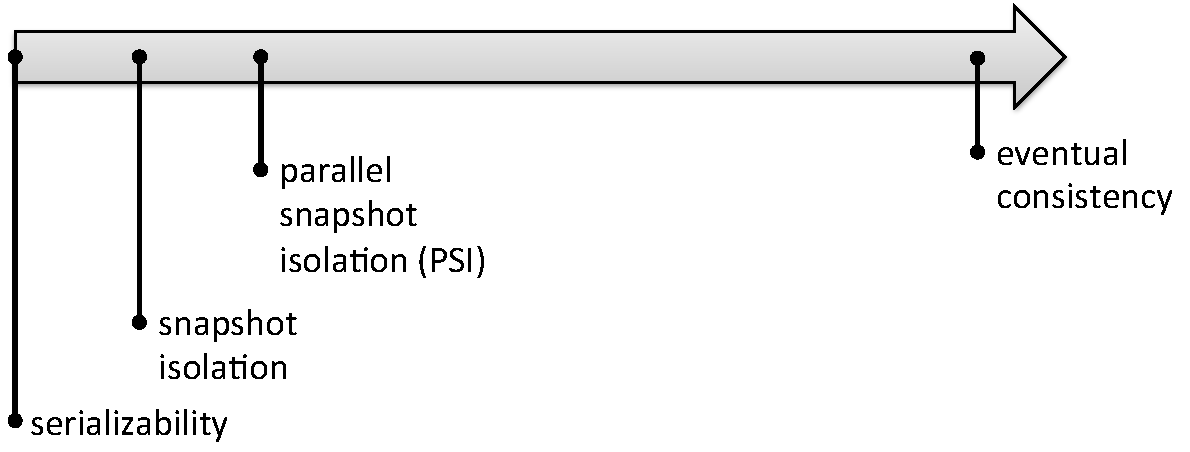
\includegraphics[width=0.5\textwidth]{figs/consistency}
\caption{Transactional Storage for geo-replicated systems from \protect\cite{Sovran:2011}}
\end{figure}

\subsection{Dependability}
	\subsubsection{Replication} % Enhance reliability and improve performance. Faul-Tolerance and Locality respectively.
	The main concerns regarding replication are at the storage layer, and there are several possible scenarios, which require each a different approach (e.g single or multi master) In the multi-master scaling is fundamental, having advantages as well as trade-offs. A good extra property to support large distributed implementations are transactions, therefore making application programming simpler without having to care about concurrency and failures, which should be dealt with at the storage layer level on each site.	
	The meaning of replication is to enhance systems reliability by having multiple copies of data at several different locations, if possible in geographically distant locations. Also, having data locality improves response times when accessing local copies of data so benefits the overall system performance implementation. There are several points to note in the following then:

\begin{itemize}
	\item{Scalability:}
	Replication is, among other things, a technique for scaling. Copying data over several locations can improve access times to local clients. A client accessing certain information can be redirected to the closest replica node available in the network of data centers. That reduces latency overhead and delays locally, although it poses a problem on the network communications required to update all other replicas once an update occurs.

	\item{Ensuring Availability and Fault-Tolerance:}
	If a replica fails there is another one which can take respond to the request and therefore avoid a single point of failure in the storage system. That creates a more robust and resilient infrastructure overall.

	\item{Load Balancing:}
	There are several strategies for that, but the most usual is having replicas located in a nearby or same data center in order to provide distribution of the incoming number of requests to the system. That approach ensures high-load peaks of requests do not overflow the systems, which is important to keep the system performing well and avoiding to slow down the processing of requests in response to clients.
\end{itemize}
	
	%\subsubsection{Availability} TODO
		
	%\subsubsection{Scalability} TODO
	
		
	%\subsubsection{Fault-Tolerance and redundancy} TODO


  %%%%%%%%%%%%%%%%%%%%%%%%%%%%%%%%%%%%%%%%%%%%%%%%%%%%%%%%%%%%%%%%%%%%%%%%%%%%%
  %
%%%%%                        LIST OF DATA STORES SECTION

%\section{Transactional support for NoSQL data stores}
\section{Typical distributed data stores in use} % list of products and their description
A full list of the types of data stores described is presented in the following sections.

\subsection{Key-Value Stores}

	\subsubsection{Voldemort}	
	Open-source follow up of Dynamo, Voldemort is being used for instance at LinkedIn for providing high-scalability. The system is built for efficient but simple queries, so there is no need or support for joins (implemented at the application level). Constraints on foreign keys are also unsupported and not possible. Obviously, no triggers or views can be set up as in traditional relational database systems. These are the trade-offs that allow the system to have better performance in terms of queries, distribution of data storage, separation of concerns between logic and data model. This is as we say, in contrast to RDBMs more practical and efficient for distributed systems with need for simple APIs and object oriented paradigms in applications.
	
	One interesting aspect of Voldemort is the concept of \emph{stores}, which are namespaces of key-value pairs stored with unique key and each of them associate to only one value. Values can be still lists, maps or scalars. In one thing it resembles Amazon Dymano, as it is highly available during write operations, can tolerate concurrency during updates and causality of versions is implemented though vector clocks.

	\subsubsection{Dynamo}
	Amazon designed Dynamo, which can also use an eventual approach but in their implementation they focused more in another type of algorithms for providing direct routing with zero hops to the destination unlike Chord~\cite{Stoica:2001}. It provides a tunable R+W \textgreater N consistency model. The application programmer using Dynamo specifies the amount of replicas that one needs up to date on a read (R) or write (W). As long as R+W is greater than N, the total number of replicas, it should provide consistency to the user (assuming correctly merged writes). That means for a typical replication factor of N=3, the programmer can specify highly available writes and slower but consistent reads (3+1\textgreater3), a more balanced approach (2+2>3), or assuming a read-heavy workload (1+3\textgreater3). Increasing N increases the replication factor, meaning better durability. Choosing \text{R+W} less or equal to N allows for eventual consistency. Although one can argue Dynamo fails to fulfil the needs of datacenters based applications.
	Most services only store and retrieve data by primary key so complex querying is not required. Consistent hashing is used for partitioning and replication. Consistency is achieved through versions of objects. Being a decentralized system, nodes can be added or removed without any extra overhead. Usually that sort of system is best for applications that need a data store that tolerates writes and there are no concurrent writes failures.
	Replication is used per node, so a coordinator node is called one upon data falls within its on range and therefore assigns copies of the source data to as many other hosts as specified by N itself.


\subsection{Document Stores}
	\subsubsection{MongoDB}
	MongoDB is one of the most popular document stores. It is schema-free and supports Map-Reduce operations too. MongoDb as well, provides indexes on collections. The consistency model is eventual and uses asynchronous replication for that. Regarding atomicity, provides atomic updates on fields by tracking changes on those and updating the whole document only if that is a known-value.
	
	\subsubsection{CouchDB}
	CouchDB on the other hand uses MVCC for atomicity on documents. Consistency is not guaranteed, each client might be having a different view of the database itself. There is no replication between replica nodes, so therefore a MVCC system to control version conflicts. It is up to the application level to handle the notifications from CouchDB for updates seen since last fetch operation.
	

\subsection{Column-Stores}
	\subsubsection{HBase}
	In previously devised systems at Google, BigTable~\cite{Chang:2006} for example mainly aims to be a highly available and scalable key-value store without compromising performance. It is then with built for lexicographically sorted data and each family has the same types. It also uses several other technologies, Chubby as a locking service, Google File Systems to store logs and data files, and SSTables for BigTable data (also implemented in HBase). In Figure~\ref{hbase-architecture} we can see an architecture design of the system developed at Google and compare it to Hbase. 

%insert figure -- %Need to explain what is metadata and put small graph maybe of BigTable?%

\begin{figure}[h]
\centering
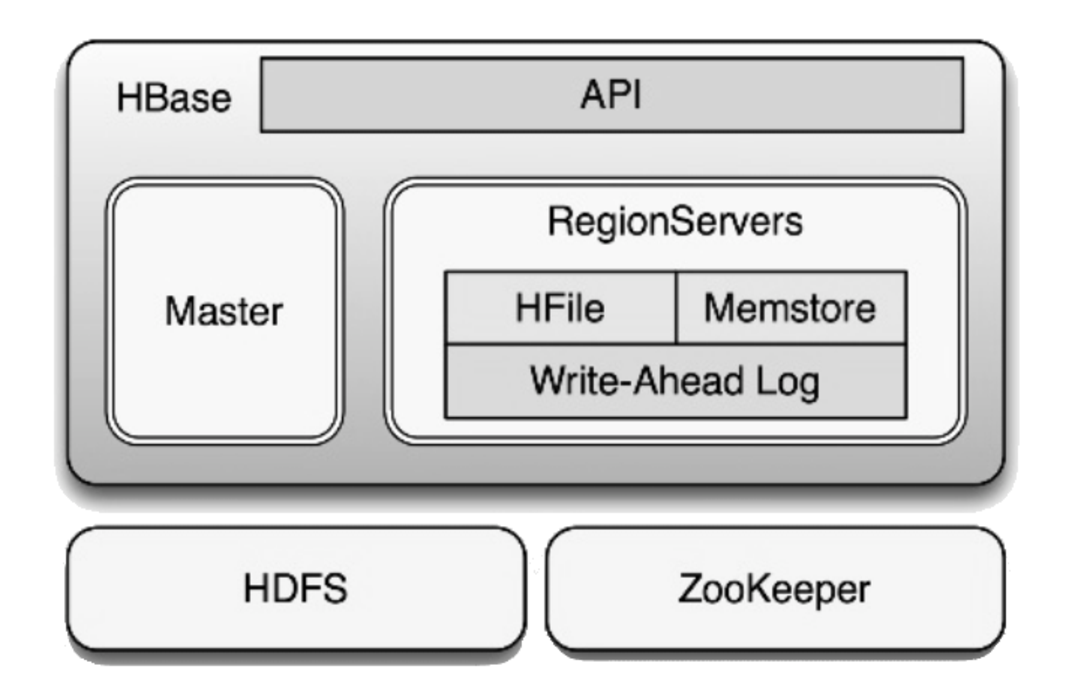
\includegraphics[width=0.5\textwidth]{figs/hbase-main-architecture}
\caption{The main HBase architecture from \protect\cite{SlidesLars}}
\label{hbase-architecture}
\end{figure}

Hbase is an open-source distributed, versioned, column-store designed after BigTable~\cite{Chang:2006}, which is also a distributed, persistent and multi-dimensional sorted map. HBase uses Zookeeper~\cite{Hunt:2010} to provide high availability and it is written in Java to managed large amounts of sparse data. The cloud data store is nowadays being used as the messaging layer at companies such as Facebook~\cite{FacebookHBase}. It has good write latency but some durability concerns (as it does not commit updates directly to disk) and not so good results in the case of reads as seen in~\cite{YCSB:2010}. The underlying file system is HDFS, analogous to GFS from Google with BigTable. In master to master replicated scenarios there are only eventual guarantees to the consistency of data, although data integrity is somehow ensured with a minimum provided set of replicas in HDFS memory of 3, claimed to be enough for the purpose.

Although that works well in most cases, more complex applications which require stronger consistency guarantees can be difficult to manage with BigTable so due to those constraints, Google developed later on in 2012 an evolution of BigTable that provided external consistency with atomic clocks and so on, Spanner~\cite{Corbett:2012}. That can make applications still benefit from high-availability while ensuring synchrony among distant replicas and more importantly, atomic schema changes. Data locality is also an important feature so partitioning of data across multiple sites is used on both BigTable and Spanner, specifically in the later to control read latency. Regarding write latency, Spanner supports that type of control by knowing how far are replicas from each other or in other words, very similarly to what had been already proposed as part of other existing middleware frameworks for HBase such as VFC$^{3}$~\cite{Vfc3:2012}.  

Performance in HBase improves as the number of servers increases due to more memory available~\cite{Carstoiu:2010}, but regardless of that fact, it is not trivial to scale always further by following the later approach. Therefore, having ways of providing different levels of consistency to users regarding data in cloud environments translates into substantial traffic savings and therefore associated costs to potential service providers or even customers, which is a very relevant matter as seen in~\cite{chihoub:2013} for consistency-cost efficiency. It is then always good to constantly be evaluating how selective replication (with a QoD in this case) can support that statement in distributed deployments with HBase.

Inside the same data center strong consistency is provided which means one can read its writes independently of what replica node is reading from. Although and as pointed out in several technical reports from Facebook~\cite{Aiyer:2012}, there is still work to do in the area of cross data center replication, which is the main aim here in the thesis work here presented and which we explain in the next chapters of the document. In master to master replicated scenarios eventual guarantees to the consistency of data are provided in HBase through mechanims based on a custom protocol with RPC calls. Therefore replicas can contain stale data in the order of seconds to minutes until the full set of updates is received.

\subsubsection{Spanner}

There has also been some recent research that addresses these shortcomings in geo-replicated data center scenarios like~\cite{Corbett:2012}. HBase does not use that Paxos either for synchronization of replicas. On the other hand, the performance of the data store for random writes and replication between remote sites is very fast and provides advantages in that area. Spanner does use Paxos for strong guarantees of replicas and that seems to work well enough, although is not really implemented with HBase it is possible to take that approach. Therefore one need to trade data availability for consistency between replicas in the presence of partitions. That is achieved through asynchronous communications rather than serializability, in order to minimize the cost of latency in wide-area scenarios with clusters running Hadoop as the storage layer of Hbase. Hadoop is good for many reasons, and frees the higher layer from other tasks and one can even implement transactions if desired on top of it.

\subsubsection{PNUTS}

On the other hand, systems as PNUTS~\cite{Cooper:2008}, yet another cloud database systems a.k.a NoSQL, Yahoo introduced a novel approach for consistency on per-record basis. Therefore being able to provided low latency during heavy replication operations for large web scale applications. They, as in our work provide a finer grain guarantees for certain data, so in other words, new updates are not always seem right away by the clients (which is the case anyway in HBase), but only if strictly necessary. Keeping that in mind, that is not always appropriate to keep the application available and performing both at once. They realize that eventual consistency is not enough in the case of social and sharing networks, as stale replicas can result in undesired cases of users having the opportunity to see or use data they were not supposed to access or so, and therefore a privacy issue as well as data consistency concerns on end users. Also, the main trade-off with PNUTS is the limited or not support for transactions.

\subsubsection{Megastore}
MegaStore is also an invention developed at Google. The main idea is to provide ACID properties across geo-located data centers with scattered data-sets and a Paxos scheme for replication. With inter data center replication Megastore can achieve fault tolerance while still providing strong consistency properties. It also scales, by partitioning data-sets into entity \emph{groups} Multi-site operations result in poor performance with Megastore, that is its main drawback. The model and language is different from those data stores such as BigTable~\cite{Chang:2006} but also from Relational Database Management Systems~\cite{RDBMS}.

\subsubsection{Azure}
There are other look alike systems such as Azure~\cite{Calder:2011} from Microsoft, which provides strong consistency on the other hand. This system tries to give priority to consistency even in the event of partitions in the network. Durability is ensured with two or more copies of the data. The systems is scalable and provides a global name-space.

Regarding its architecture, Storage Stamps are used to expand out global data center capacity. The Geo-Location service does the balancing and fail-over across different stamps across different data centers. Within a Storage Stamp, there is a Stream Layer which is append-only distributed file system which replicates data across domains. Replica recovery is possible. The Partition Layer understand what is a data structure is (blobs, queues..) and it is possible to manage the consistency of the items in the Stream Layer (persistence). Basically, the partition layer sends asynchronously the items for geo-replication. There is also a commit log similarly to the WAL in HBase, which is useful for recovery in case it is necessary.

\subsubsection{Cassandra}
Cassandra is a well known key value store system developed at Facebook for scaling of their back-end storage architecture while achieving high performance and wide applicability~\cite{Lakshman:2010}. Replication is support across multiple data centres, providing quite low latency for reads and specially writes. The key point of Cassandra is its ability to define several types of consistency, which can be configured by the user before runtime. Cassandra works similarly to HBase, using a write ahead log for durability and a Memtable to store volatile data. Atomicity is ensure at the row-level, which is none or nothing. As we we will see later in our implementation of HBase QoD, Cassandra uses a tunable data consistency model which also works for distributed environments. 

\paragraph{Scalability:}
To scale Cassandra follows a similar approach to Chord~\cite{Stoica:2001}, where the load is partitioned among the neighboring nodes to avoid the load goes on some of the existing nodes only.

\paragraph{Fault-Tolerance:}
Cassandra uses replication Quorums for ensuring data is fault tolerant. In the replication model, either all nodes respond for the write to be successful or none of them does. Read-repair occurs when obsolete data must be updated in a per request basis. That is data that will need to be up to date for an eventual "Insert", "Update" or similar operation on the database.

% Quorum -> replication factor
% 4 -> duplicate in every row
% 3-> must respond for write to be successful
%
%All -> respond from all the nodes managing information for write to be successful.

%Fault-Tolerance:
%If am writing some data in the node, 

%Read-repair ensures that obsolete data is updated in a request basis. That data will be up to date. Select, Insert, ...

\subsection{Other related approaches}
\subsubsection{Google Cloud Data Store}
Google Cloud Datastore has been recently released. That is a system that is subject to exploration yet so we will cover limited aspects of it here. The API enables users to use a a fully managed, schemaless database on the cloud for storing their non-relational data.

There are a few key points such as ACID properties of transactions or High-Availability, Google outlines in their main website~\cite{GoogleCloudDataStore}. More interestingly also provides a differentiated approach to consistency. Strong consistency for certain reads and eventual for the rest of the queries. The reason for giving stronger consistency to some queries over others with just eventual is allowing the database performance to optimize on the overhead of strong consistency between groups of non-related items. To the contrary, with related entities, such as [Person:GreatGrandpa, Person: Grandpa, Person:Dad, Person:Me] it is by default possible with ancestor queries to use stronger consistency. Transactions are also implemented between entity groups to ensure data consistency in cases of concurrent updates to the database. As they note, to conserve memory a query should, whenever possible, specify a limit on the number of results returned, that is why.

To us, this concept is also interesting as it seems to make use of the right tools depending of what type of data is being used in order to maintain as much consistency as possible at a low-cost.

\subsubsection{MapReduce Framework}
In the MapReduce framework~\cite{Dean:04}, replication is used for tolerating failures and also performance wise. The framework was first introduced by Google and used and underlying file system called Google File System (GFS)~\cite{Ghemawat:03}. Here files are organized into chunks which are replicated to other nodes for fault-tolerance. The processing of map tasks involves the task scheduler and it is performed leveraging data locality information kept in the metadata storage, for instance first asking for the chunks required to complete tasks at the current node, in another in the same location (data center) or else outside in a completely different location, in that order of priority. That also ensures fault-tolerance and improves task average time completion by using more nodes with the relevant data available in order to speed up the process by contributing to the overall computation in parallel with the rest.


  %
 %%%
%%%%%                           THE END
  %
  %%%%%%%%%%%%%%%%%%%%%%%%%%%%%%%%%%%%%%%%%%%%%%%%%%%%%%%%%%%%%%%%%%%%%%%%%%%%%
                    	% state of the art

  %%%%%%%%%%%%%%%%%%%%%%%%%%%%%%%%%%%%%%%%%%%%%%%%%%%%%%%%%%%%%%%%%%%%%%%%%%%%%
  %
%%%%%               P A R T   I I I  --  Implementation
 %%%
  %

%\part{Part}
\thispagestyle{empty}
%\vbox to\textheight{
%\vfil
%\chapter*{The System}
\thispagestyle{empty}

%In this part of the thesis we focus mainly in our system and its technical characteristics, implementation details and relevant points to integrated it into the target architecture, HBase in that case.

%}
%
\newpage
\thispagestyle{empty}
\chapter{Architecture}
\label{ch:architecture}

\begin{quotation}
“The greatest pleasure in life is doing what people say you cannot do.”
{\small\it -- Walter Bagehot (British political Analyst, Economist and Editor, one of the most influential journalists of the mid-Victorian period.1826-1877) }
\end{quotation}

This chapter explains the design goals, main architecture, and the protocols we present as solution to the problem of distributed data stores regarding consistency versus availability, also introduced in earlier chapters. Rather than just considering a fixed consistency model, we aim at providing finer-grained levels of consistency during data replication, and taking as an example social networks such as Facebook~\footnote{http://www.facebook.com}, we showcase how one might not need so strict consistency depending on what updates are replicated. For that, will be explored how bounded data semantics help to achieve that goal.

First of all, we take a general overview of the system design in Section~\ref{architecture:overview}. Following sections in the chapter reflect the architecture of the system in terms of network as well software components. Each of the steps in the design process has been carefully justified in order to integrate well in the original system architecture, and in particular those decisions related to asynchronous replication using Remote Procedure Call~\footnote{RPC, http://en.wikipedia.org/wiki/Remote\_procedure\_call} mechanisms that are the base of the architectural changes introduced with a custom HBase-QoD module.


%% **** TODO STOP *** rewrite chapter overview

In order to achieve that, it is necessary to take into account a set of requirements that help at addressing the challenges and fulfilling our goals, that are described  in Section~\ref{architecture:requirements}. Section~\ref{architecture:network} presents the network architecture where HBase-Qod operates. In Section~\ref{architecture:consistency}, we describe the consistency model proposed for HBase-QoD, including operation grouping, and its enforcement. The chapter closes with the software architecture of the extensions proposed to HBase.


  %%%%%%%%%%%%%%%%%%%%%%%%%%%%%%%%%%%%%%%%%%%%%%%%%%%%%%%%%%%%%%%%%%%%%%%%%%%%%
  %
%%%%%                        SECTION
 %%%
  %

% How the containers replicate thigns with the QoD
%reprise overall system overview of HBase (if needed check approach in papers such as BigTable or HBase papers/docs) kind of usage overview, applications, storage, data centers, etc. (the 1000 feet view or birds-eye view)



\section{System Architecture Overview}\label{architecture:overview}
%%%% TODO STOP REWRITE THIS TEXT FOLLOWING THE NEW STRUCTURE OF THE CHAPTER
We start by showing the logic behind the main architectural design decisions and showcase scenarios as in a "thousand feet view" of the system, which provides an overview of the system first of all such as in Figure~\ref{fig-high-level}. Following, we delve into the proposed changes in order to verify the feasibility of the implementation as well as what scenarios are best suited to our definition of consistency.

%insert 1000 feet view
\begin{figure}[h]
\centering
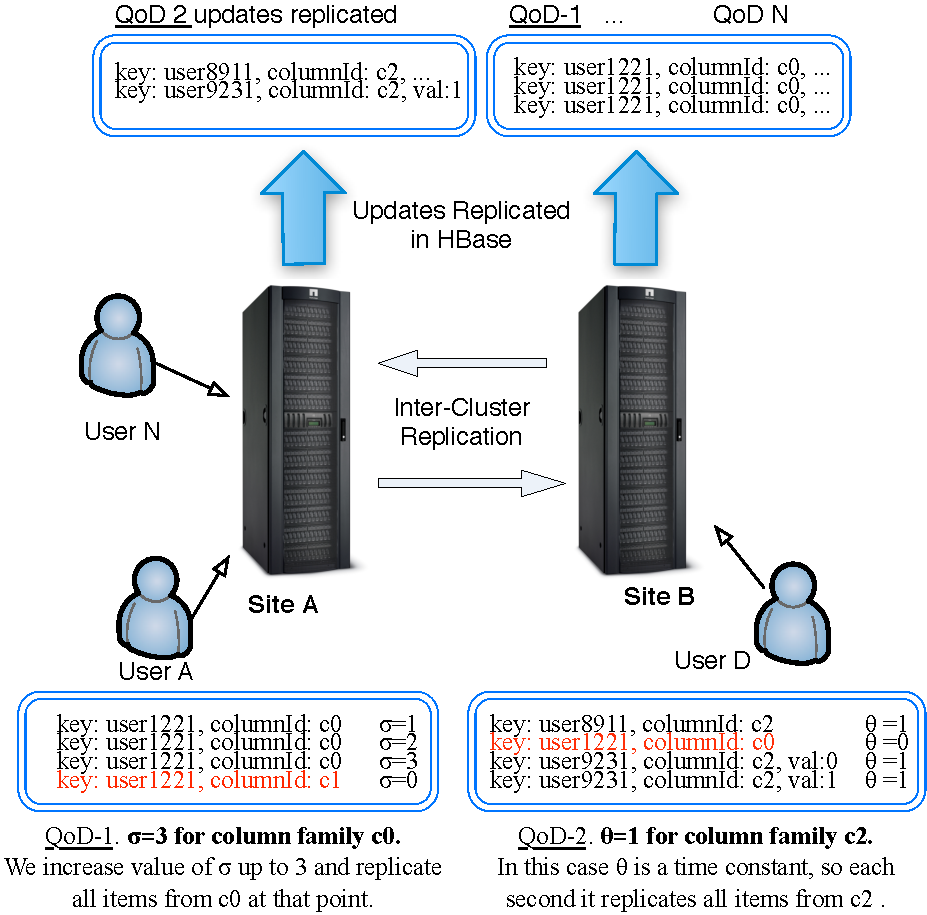
\includegraphics[width=0.8\linewidth]{figs/highlevel.pdf}
\caption{HBase QoD high-level}
\label{fig-high-level}
\end{figure}


In order to introduce a new HBase-QoD module architecture, the first step is to study in details the existing system to get familiar with it and identify the best locations for new code added. Therefore, taking into account the original architecture inner-workings of the data store at the logical level will ensure correctness and validity of the new architecture here presented as well as prototype described in next chapter.

\begin{enumerate}
\item First identifying the source and destination of updates.
\item Secondly, defining a QoD vector-model based on the schema design of HBase so we can reach our goals.
\item Finally integrating both parts into the same system, and providing a mechanism to switch on and off the module at run time into HBase.
\end{enumerate}

% Implementation details, such as WALEdit, algorithm, images of QoD inside DC, etc.
HBase is written in Java and its replication mechanisms are related to a Write Ahead Log (WAL) that also ensures durability of updates and disaster recovery. Replication must be enabled for shipping updates between peer cluster locations in remote or nearby data centers. The process of replication is carried out asynchronously so there is not additional overhead or latency introduced in the the master server during that operation.  Although, since the process is not strongly consistent, in write heavy applications a slave can have stale data in the order of more than just a few seconds according to the eventual consistency approach.

Therefore, until the last update first commits to the local disk, it cannot be seen replicated in a remote location. To keep control of staleness, we plug a QoD module called HBase-QoD which provides and takes advantage of a filtered and sorted by priority queue of items later scheduled for replication accordingly. Thereafter, when the method completes, updates are shipped in an ordered fashion by defining and enforcing bounds on data as key decision properties for their delivery to a remote cluster location. For write intensive applications that can be both beneficial in terms of peaks of bandwidth usage and also reduced staleness of data.

Given that HBase provides eventual consistency mechanisms through Remote Procedure Calls in order to replicate items, that data store is chosen as system use case to firstly introduce the proposed architecture here. Also, we can enhance the current multi-row atomic model, using an approach that can also relate column families between updates in order to provide the same atomicity at the column-level.

%\paragraph*{Data Center Storage View:}
The physical structure of column families is outlined in Table~\ref{tab:hbase-model}, where we have a view of its data model. That is potentially useful for distinguishing updates between cluster update owners and users or applications that need those updates from another cluster for the fact of being consistently up to date in regards to their own local data center ongoing update operations.

%The overall architecture layout is presented in Figure~\ref{fig-high-level}. The module that introduces the vector-field consistency model is shown in Algorithm~\ref{algo1}, and follows the architectural design choices of HBase as well as the main goals here desired. In addition to that, in Section~\ref{grouping} we also explain how to group updates and what are the benefits of doing that.

%\paragraph*{Replication Flow:}
Replication occurs in two different manners into HBase. Intra-cluster and Inter-Cluster. We target the later, so firstly, we set up a standalone Zookeeper~\footnote{http://zookeeper.apache.org/} on each server running, and therefore separate clusters with a master server each. This is useful for enabling and testing HBase-QoD performance.

Secondly, a cluster with a distributed Zookeeper ensemble on each of the nodes is configured, and we will aim to also test intra-cluster scenarios for HBase-QoD even though that is not our main goal. This benchmark use case can be also useful to us for testing weak consistency features presented into YCSB++\footnote{http://www.pdl.cmu.edu/ycsb++/}.

%\paragraph*{Usage}
%The usage of HBase-QoD is straight-forward and integrated into HBase core architecture. % keep writing here about cli possible function (ruby)
%The configuration for that is shown in the following Figure~\cite{}

\begin{center}
\begin{table}\label{tab:hbase-model}
\centering
\begin{tabular}{ |l|l|l|l| }
\hline
Row Key & Timestamp & Column & Value \\ \hline
\multirow{3}{*}{com.gsd.inesc-id.www} & T1 & anchor:inesc-id.gsd.com & value1\\
 & T1 & anchor:domain2.com & value2\\
 & T2 & anchor:domain3.com & value3\\
 \hline
\end{tabular}
\caption{This table shows the physical structure of HBase data model}
\end{table}
\end{center}



%%%%%%%%%%%%%%%%%%%%%%%%%%%%%%%%%%%%%%%%%%%%%%%%%%%%%%%%%%%%%%%

\section{From eventual consistency to QoD consistency}\label{architecture:requirements}
This section explains the motivation of the steps taken in regards to the design decisions adopted in order to present an enhanced architecture that also follows best practices in regards to code readability and re-usability for the system of choice. In the following sections of the chapter we justify the 'how' and 'why' of the choices we have made during the development process later once we have a well-rounded architecture of the intended replication module for HBase.

With eventual consistency enforcement in place, updates and insertions are propagated asynchronously between clusters so Zookeeper is used on each of them for storing their positions in log files that hold pointers to the next log entry to be shipped when replicated from/to other HBase cluster. To ensure cyclic replication (master to master) and prevent from copying same data back to the source, a sink location with remote procedure calls invoked is already into place with HBase, so we use the current features provided by HBase in that regard. Therefore if we can control the edits to be shipped, we can also decide what is replicated, when or in other words, how soon or often.

Design Goals are as follows:

\begin{enumerate}
\item Separation of concerns between replication data semantics. Applied to HBase can provide different levels of consistency among updates.
\item Replication can be still asynchronous but with higher degree of consistency guarantees, based on a vector-field consistency model that allows defining constraints and limits applied to updates that have as target different client application data.
\item Partitioning allowed with eventual consistency allowing to reconcile changes autonomously, while grouping of operations enforces maintaining atomically replicated updates so avoiding the first in case of long periods of disconnection to the network (it is already possible to define a retry timeout in HBase in case of partitioning so we do not need to focus on that but rather on the grouping part)
\end{enumerate}

\subsection{Challenges addressed in HBase-QoD}

How long does it take for edits to be propagated to a slave cluster? This is one of the main questions that can strike Cloud Architects when it comes to distributed NoSQL architectures. As noted in the HBase forums, there is a increasing interest in knowing how and when data is propagated to slave clusters. For instance to separate clients facing HBase clusters and the ones used to to run benchmarks and analysis that involves heavy Map Reduce tasks that are very scan intensive.

\paragraph*{Buffering in HBase:}
As noted by Jean-Daniel Cryans, replication acts as soon as the buffer itself is full or it reaches the end of the file (EOF). The end of a file is determined by when a file is reopened because there is no way to tail a file into HDFS without closing a previous reader, therefore reopening the file and seeking to a certain position it is required. As a consequence, replication is not able to keep filling the buffer for minutes before sending because it quickly gets to the end of the file anyway. The HBase replication stream is almost always in the range of sub-seconds lag. Only if it reaches the end of a file and it does not read anything new, then that will be waiting for new updates to arrive.

In the case of \emph{ReplicationSource}, that tails the WAL and sends the WALEdit to the ReplicationSink via RPC. In other words, the code applies the edits to the slave cluster via a remote call to the method in the RPC sink (calling a method named \emph{ReplicateLogEntries} remotely).

In order to control that, HBase-QoD modifies the internals of buffering WALs at the source that will be sent to a sink location.

\paragraph*{Configurations:}
There is a set of configurations in HBase to control how updates are replicated. That is contained in XML file called hbase-site.xml.

\begin{enumerate}
\item replication.source.size.capacity, default is 64MB but recently so that is possibly too big.
\item replication.source.nb.capacity, default is 25k. The buffer is flushed when either size or capacity is reached but what really important is the size.
\item replication.source.maxretriesmultiplier, default is 10, so it retries up to 10 times with pauses that are currentIteration times.
\item replication.source.sleepforretries. By default it sleeps 1 sec, 2, 3, 4... 9, 10, 10, 10, 10 until it's able to replicate (default is 1)
\end{enumerate}

Although useful, currently those mechanisms do not allow differentiation between data priority when it comes to flushing updates to slave cluster. Therein HBase-QoD described next is devised to see how it can help in that regard.


%%%%%%%%%%%%%%%%%%%%%%




  %%%%%%%%%%%%%%%%%%%%%%%%%%%%%%%%%%%%%%%%%%%%%%%%%%%%%%%%%%%%%%%%%%%%%%%%%%%%%
  %
%%%%%                        SECTION
 %%%
  %

\section{Network Architecture and Protocols}\label{architecture:network}
% - diagrams and clear explanations of how HBase and its distribution and replication works within data center and across data centers this is where your diagrams should show up describing the information flows and where QoD is to be applied.
At the Replication Level, the network architecture is as shown in Figure ~\ref{fig-replication-level}. Which reflects the main components at each site by exposing them into adjacent layers which interact with each other. The flow is both, upwards and downwards the stack in each of the Master servers of HBase in the distributed cluster set up at INESC-ID.

\begin{figure}[t]
\centering
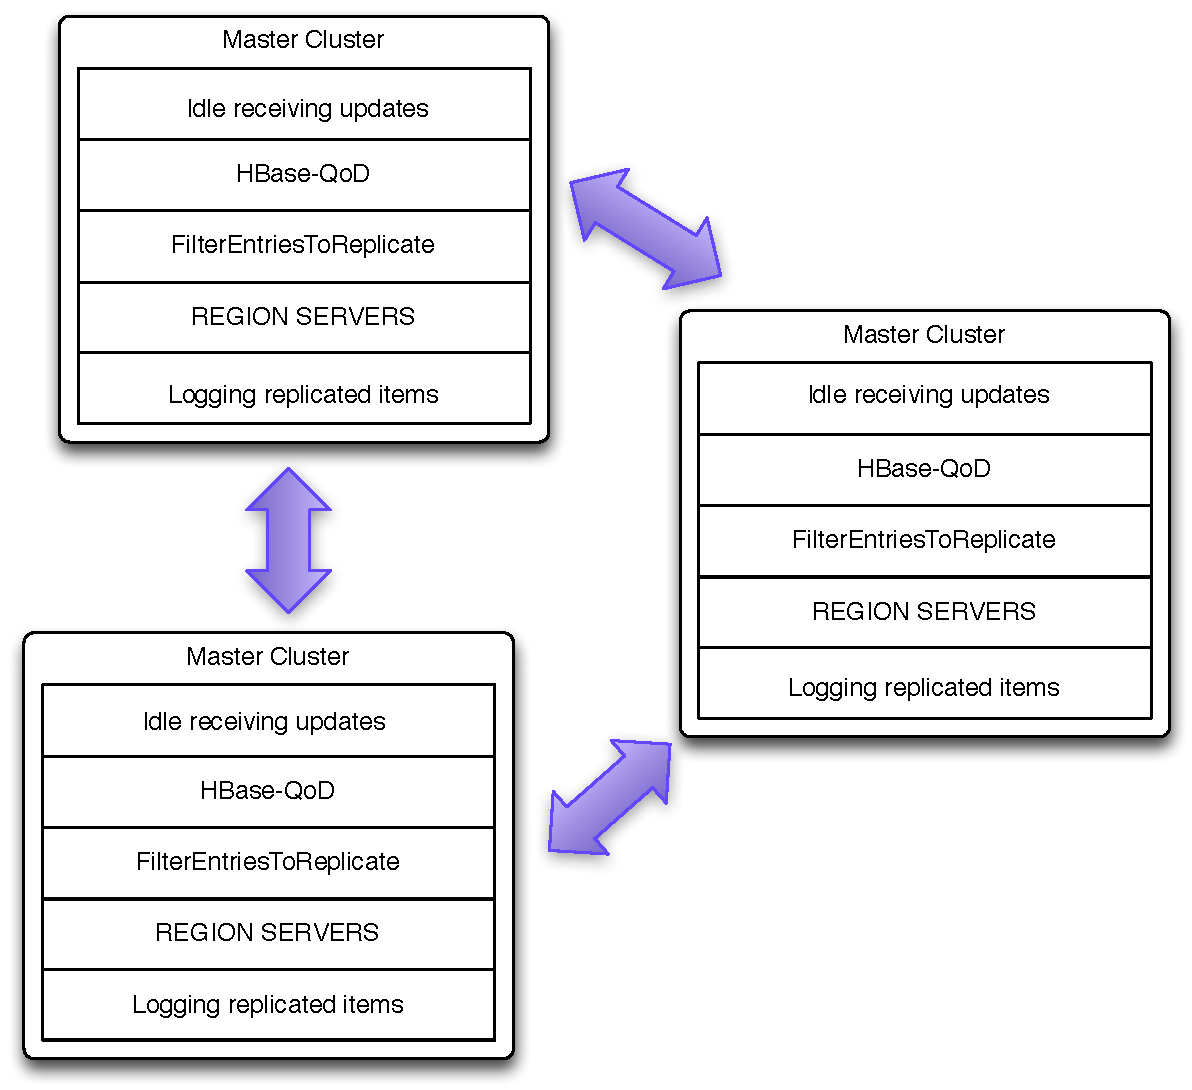
\includegraphics[width=0.8\linewidth]{figs/ReplicationFlow.pdf}
\caption{Replication Flow of updates}
\label{fig-replication-level}
\end{figure}

%\paragraph*{*****Prototypical Example}
% complete example of usage, that I think you are presenting in the implementation. describe how a client application program  can specifiy the Qod and operationg groupings so that the reader sees everything now in a complete example (this may be shown earlier but I think it is a good way of wrapping up everything and make it more clear)
We extend HBase, adding updates due to be replicated in a priority queue according to their own QoD in each case. Thereafter once the specified QoD threshold is reached another thread from HBase in the form of Remote Procedure Call collects and ships all of them at once.

\begin{figure}[t]
\centering
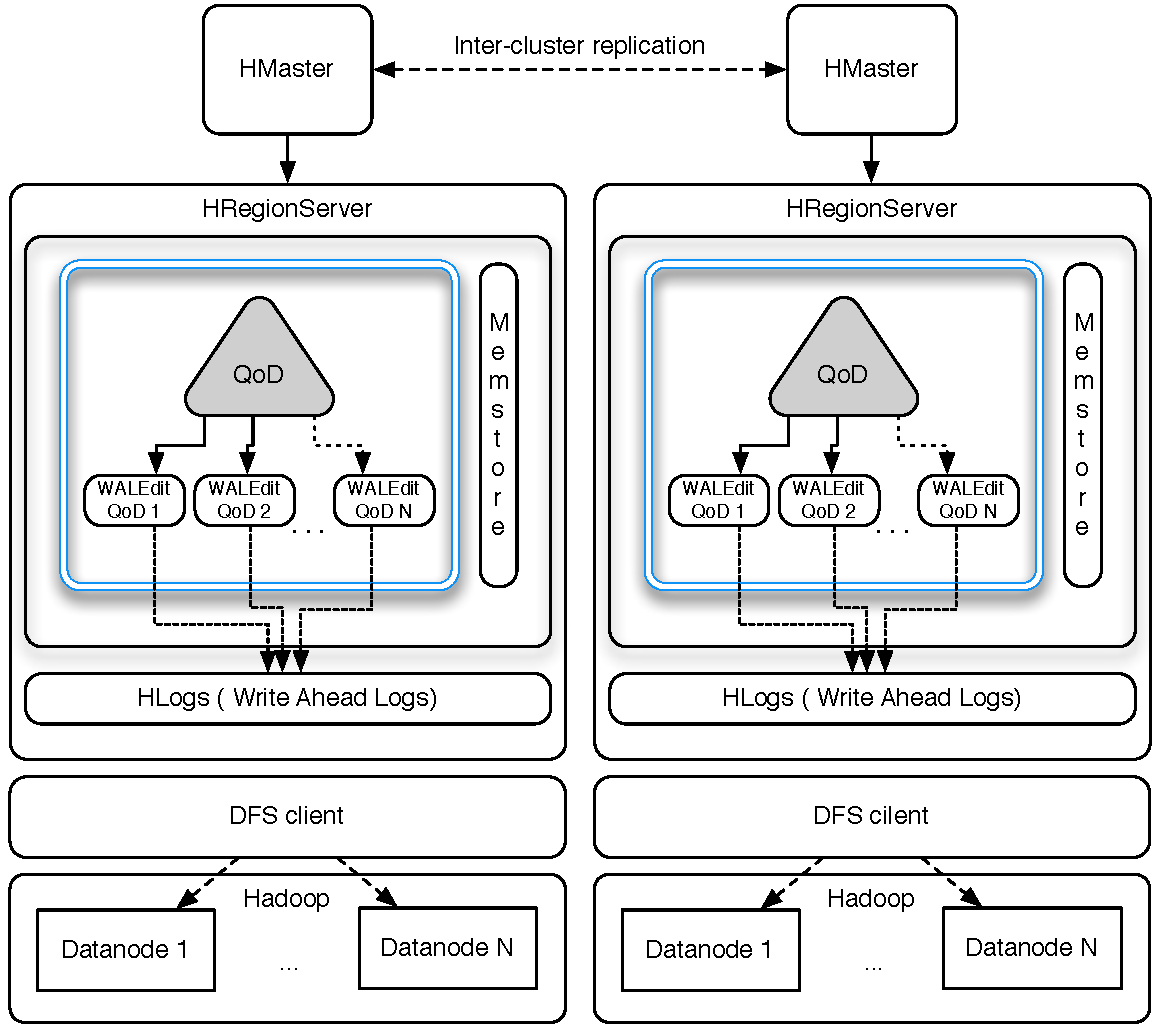
\includegraphics[width=0.8\linewidth]{figs/multi-site.pdf}
\caption{HBase QoD operation}
\label{fig-qod-module}
\end{figure}

In Figure~\ref{fig-qod-module} we observe the QoD module plugging into HBase, intercepting the incoming updates from the upper layers and passing them down and the resulting outcome to the Write Ahead Logs for later replication.

%\paragraph*{Remote Procedure Calls}
HBase implements remote procedure calls for the replication of items between servers or clusters. These mechanisms have been proven a useful paradigm for providing communication across computer networks for several reasons~\cite{Birrell:1984}. An RPC mechanism is mainly responsible for providing control of data transfers between a source and a destination location. In the case of HBase, these are called \emph{ReplicationSource.java} and \emph{ReplicationSink.java} respectively. To understand in depth that topic, it has been discussed in as much depth as possible with Apache Foundation contributors for the HBase community. That is helpful to clarify and understand better how the system operates before introducing the changes proposed with our HBase-QoD.



%\section{System Architecture}
% architecture inside each HBase instance with your new modules.
%A three-dimensional vector constraint model based on~\cite{Santos:2010} is implemented in the form of the corresponding QoD paradigm, shipping updates for replication, or retaining them for later shipment as mentioned. For that to be possible, we have used a set of customized data structures, which hold the values of the database rows we desire to check according to some specific field we might be interested in (e.g column family) for replication.

\section{QoD Consistency Enforcement}\label{architecture:consistency}
% description of the VFC algorithms and how the consistency is enforced whan updates arrive , etc. this also includes operation grouping (only code like details should be left for the implamentations, e.g., the listings that you show there and are ok).
%% Start by presenting our model, constraints, data containers, and how things work (are enforced / evaluated )

Consistency enforcement in HBase-QoD is inspired in three-dimensional vector constraint model based on~\cite{Santos:2010}, and adapted to HBase in order to drive shipping updates for replication, or retaining them for later shipment as mentioned. For that to be possible, we have used a set of customized data structures, which hold the values of the database rows we desire to check according to some specific field we might be interested in (e.g column family) for replication.

The QoD paradigm implemented allows for entries to be evaluated prior to replication based on one or several of the three parameters in a three-dimensional vector K ($\theta$, $\sigma$, $\nu$), corresponding to Time, Sequence, Value respectively in our case. Secondly, we take care of updates that collide with previous ones (same keys but different values). They can also be checked for number of pending updates or value difference from previously replicated updates, and then shipped or kept on the data structure accordingly. The time constraint can be always validated every X seconds, and the other two constraints are validated through Algorithm.~\ref{algo1}, whenever updates arrive. For the work presented here we use Sequence ($\sigma$) as the main vector-field bound (\texttt{HBaseQoD.enforce(containerId)}).

% architecture inside each HBase instance with your new modules.
The original HBase architecture has built-in properties derived from the underlying HDFS layer. As part of it, the WALEdit data structure is used to store data temporarily before being replicated, useful to copy data between several HBase locations. The QoD algorithm (shown in Algorithm.~\ref{algo1}) uses that data structure, although we extend it to contain more meaningful information that help us in the management of the outgoing updates marked for replication.

% High-level algorithm we use to modify queued items for replication
\begin{algorithm*}
\caption{QoD high-level algorithm for filtering updates}
\label{algo1}
\begin{algorithmic}[1]
\REQUIRE $containerId$
\ENSURE $maxBound \neq 0$ and $controlBound \neq 0$
%\STATE $y \leftarrow 1$
\WHILE{$enforceQoD (containerId)$}
\IF{$getMaxK(containerId) = 0$}
\RETURN $true$
\ELSE[$getactualK(containerId)$]
\STATE $actualK(\sigma) \leftarrow actualK(\sigma)+1$
	\IF{$actualK(\sigma) \geq containerMaxK(\sigma)$}
	\STATE $actualK(\sigma) \leftarrow 0$
	\RETURN $true$
	\ELSE
	\RETURN $false$
	\ENDIF
\ENDIF
\ENDWHILE
\end{algorithmic}
\end{algorithm*}

To compare and track the QoD fields, that act as constraints to replicate updates, against these stored entries, we defined data \emph{containers} which are useful to keep track of the current value of the vector-field selected to bound replication to, and secondly the maximum value it will be allowed to reach before updates are flushed to the slave cluster and then reset again. That is as what we call the QoD percentage of updates replicated (according to the selected vector-field bound, e.g $\sigma$). The process is partly automated, of by now, we just define it at run-time (or by the developer later) by adding a parameter into the system console to define a vector-field specific bound.

\subsection{Caching updates}\label{architecture:caching}
The problem with controlling the flow of updates for shipping through replication is indeed what to do with them until one is able to handle them appropriately. Therefore it is devised a \emph{Unified Caching} layer into HBase-QoD, which serves as a helper to keep track of items and their priority for replication. When an update is received and the QoD bound is reached, the Cache is either emptied and updates are shipped or it is starting to be filled again. That allows to differentiate between \textbf{Critical} and \textbf{Non-Critical} updates.

\subsection{Operation Grouping}\label{grouping}
At the application level, it may be useful for HBase clients to enforce the same consistency level on groups of operations despite affected data containers having different QoD bounds associated. In other words, there may be specific situations where write operations need to be grouped so that they can be all handled at the same consistency level and propagated atomically to slave clusters. 

For example, publication of user statuses in social networks is usually handled at eventual consistency, but if they refer to new friends being added (e.g., an update to the data container holding the friends of a user), they should they should be handled at a stronger consistency level to ensure they are atomically visible along with the list of friends of the user in respect to the semantics we describe here.

In order to not violate QoD bounds and maintain consistency guarantees, all data containers of operations being grouped must be propagated either immediately after the block execution, or when any of the QoD bounds associated to the operations has been reached. When a block is triggered for replication, all respective QoD bounds are naturally reset. 

To enable this behavior we propose extending the HBase client libraries to provide atomically consistent blocks.
Namely, adding two new methods to HTable class in order to delimit the consistency blocks: \textit{startConsistentBlock} and \textit{endConsistentBlock}. Each block, through the method \textit{startConsistentBlock}, can be parameterized with one of the two options: i) \textit{IMMEDIATE}, which enforces stronger consistency for the whole block of operations within it; and ii) \textit{ANY}, which replicates a whole block as soon as any QoD vector field bound, associated with an operation inside the block is reached.

Next, in Listing~\ref{lst:group-listing} we provide an illustrative simple example of a social network where three containers with different consistency levels are modified. Note that we are not aiming at full transactional support, as it would be possible to change the same data containers modified by a set of grouped operations, at the same time, from other operations individually.

\begin{lstlisting}[language={java}, caption={Operation grouping},label={lst:group-listing}]
htable.startConsistentBlock(ConsistencyType.IMMEDIATE)
Put put1 = new Put(Bytes.toBytes("row1"));
put1.add(Bytes.toBytes("SocialNetTable"),Bytes.toBytes("status"), Bytes.toBytes("friend 12345 added"));

Put put2 = new Put(Bytes.toBytes("row2"));
put2.add(Bytes.toBytes("SocialNetTable"), Bytes.toBytes("friends"), Bytes.toBytes("12345"));

Put put3 = new Put(Bytes.toBytes("row3"));
put3.add(Bytes.toBytes("SocialNetTable"), Bytes.toBytes("wall"), Bytes.toBytes("12345 is now a friend"));

htable.put(put1);
htable.put(put2);
htable.put(put3);

htable.endConsistentBlock();
\end{lstlisting}

\subsection{Proposed scenario}
One of the key factors for having operations grouping working together with HBase-QoD is the depicted in Figure~\ref{fig-qod-grouping}. We can see that the operations that are grouped need to communicate over the network less often to other clusters, while arriving earlier in some cases than updates shipping as if several individual operations from location Cluster A were performed. This is due to the ability of HBase-QoD to deliver demanded updates in a consistent timely-fashion rather than on a per request arrival basis, which means possibly delaying the replication process by a fraction of the amount of communication that can be saved instead using the mentioned technique.

\begin{figure}[t]
\centering
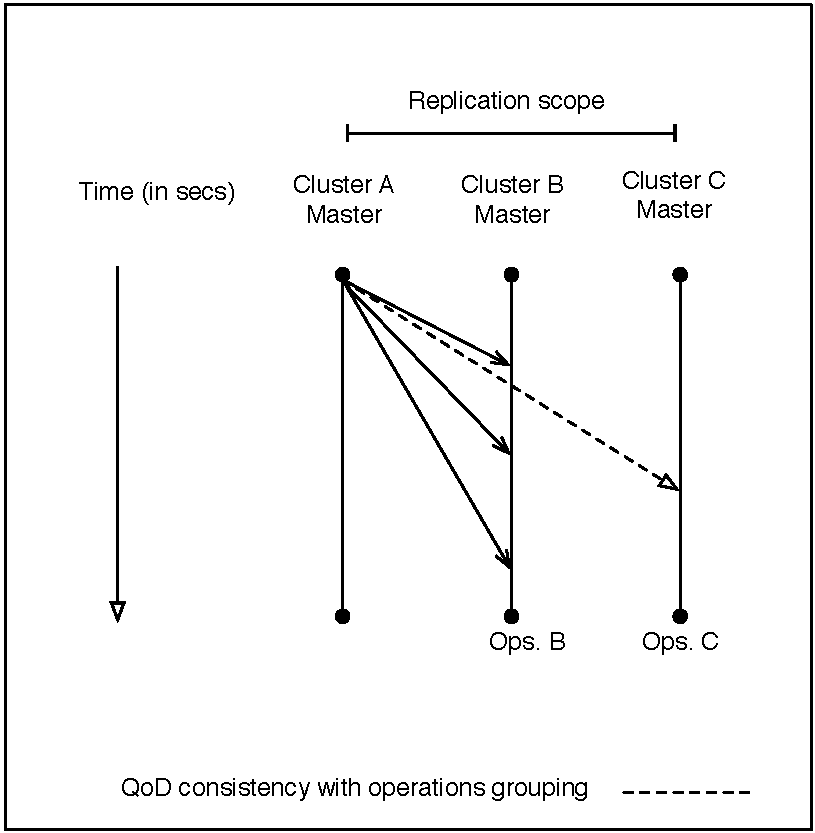
\includegraphics[scale=0.6]{figs/operation-grouping.pdf}
\caption{Resulting scenario of grouping operations in a time-lined based diagram using HBase-QoD versus a regular HBase deployment at Cluster B}
\label{fig-qod-grouping}
\end{figure}

Another experiment that has been conclusive in terms of grouping of operations is the comparison between different QoD levels, in the case of values for vector field K (-, $\sigma$, -). Setting the operation grouping for a small number of updates still shows that a timestamp in the receiving server is the same for every item in the group. The following set of operations is reflect in Figures~\ref{fig-shipping-grouping} and ~\ref{fig-receiving-grouping}. The same principle can be applied and has been demonstrated to work in the same fashion for different sets of containers.

%(table_name::columnFamily).

\begin{figure}[b]
\centering
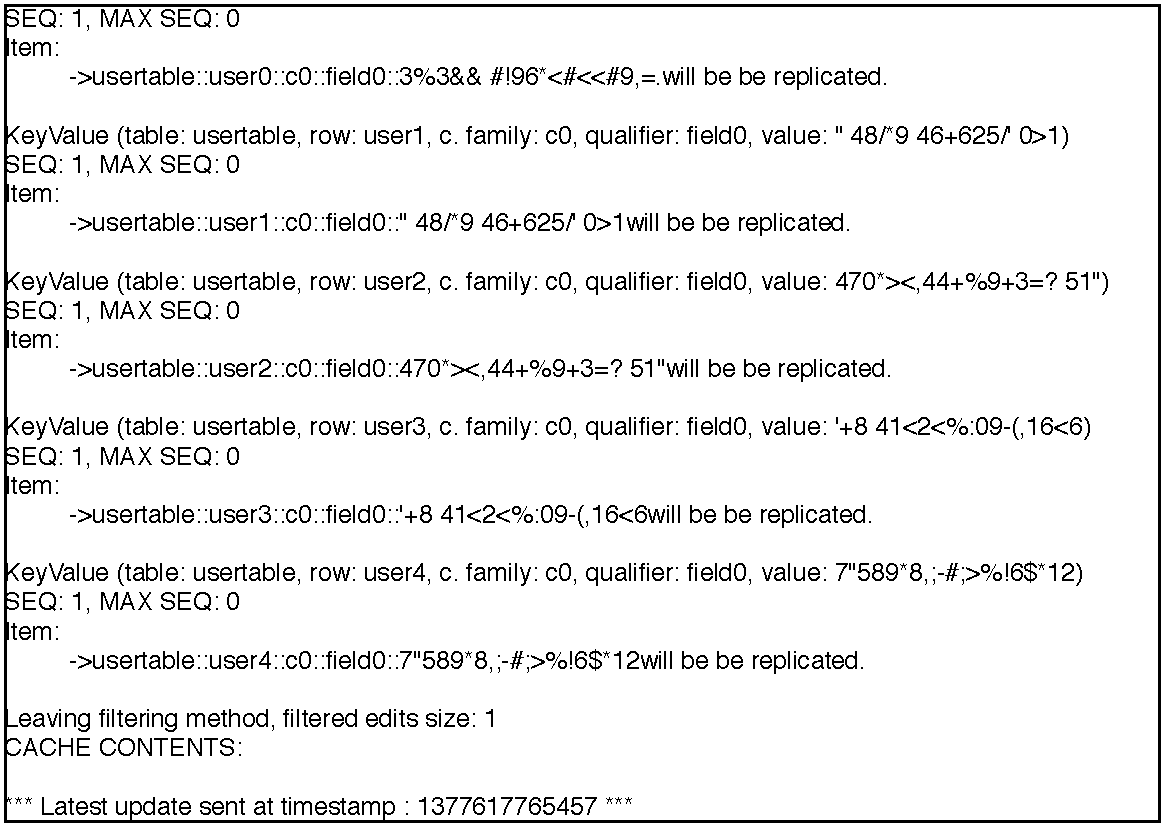
\includegraphics[scale=0.6]{figs/ginja2-grouping-send.pdf}
\caption{Sending from ginja-a2 to ginja-a1}
\label{fig-shipping-grouping}
\end{figure}

In the following Figure~\ref{fig-receiving-grouping}, we observe how the timestamp for each of the items replicated from the grouped operation have the same timestamp (\textbf{1377617765557}) at the receiving side on ginja-a1. That ensures they have arrived at the same time, and actually we verify the correctness of the experiment by leveraging internal HBase mechanisms that are currently being already used to list statistics of the age of updates sent and/or receive. At the sending side on the other hand, each update is grouped until finally they are all due to be replicated as a whole and therefore printing the timestamp only in order to comply with the reality.

\begin{figure}[t]
\centering
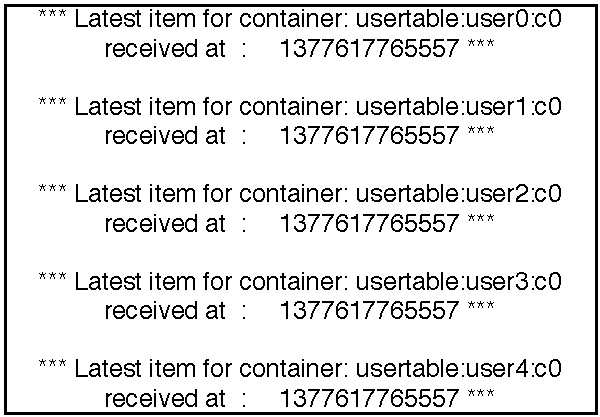
\includegraphics[scale=.6]{figs/ginja1-grouping-receive.pdf}
\caption{Receiving from ginja-a2 in ginja-a1}
\label{fig-receiving-grouping}
\end{figure}





\begin{figure}
\centering
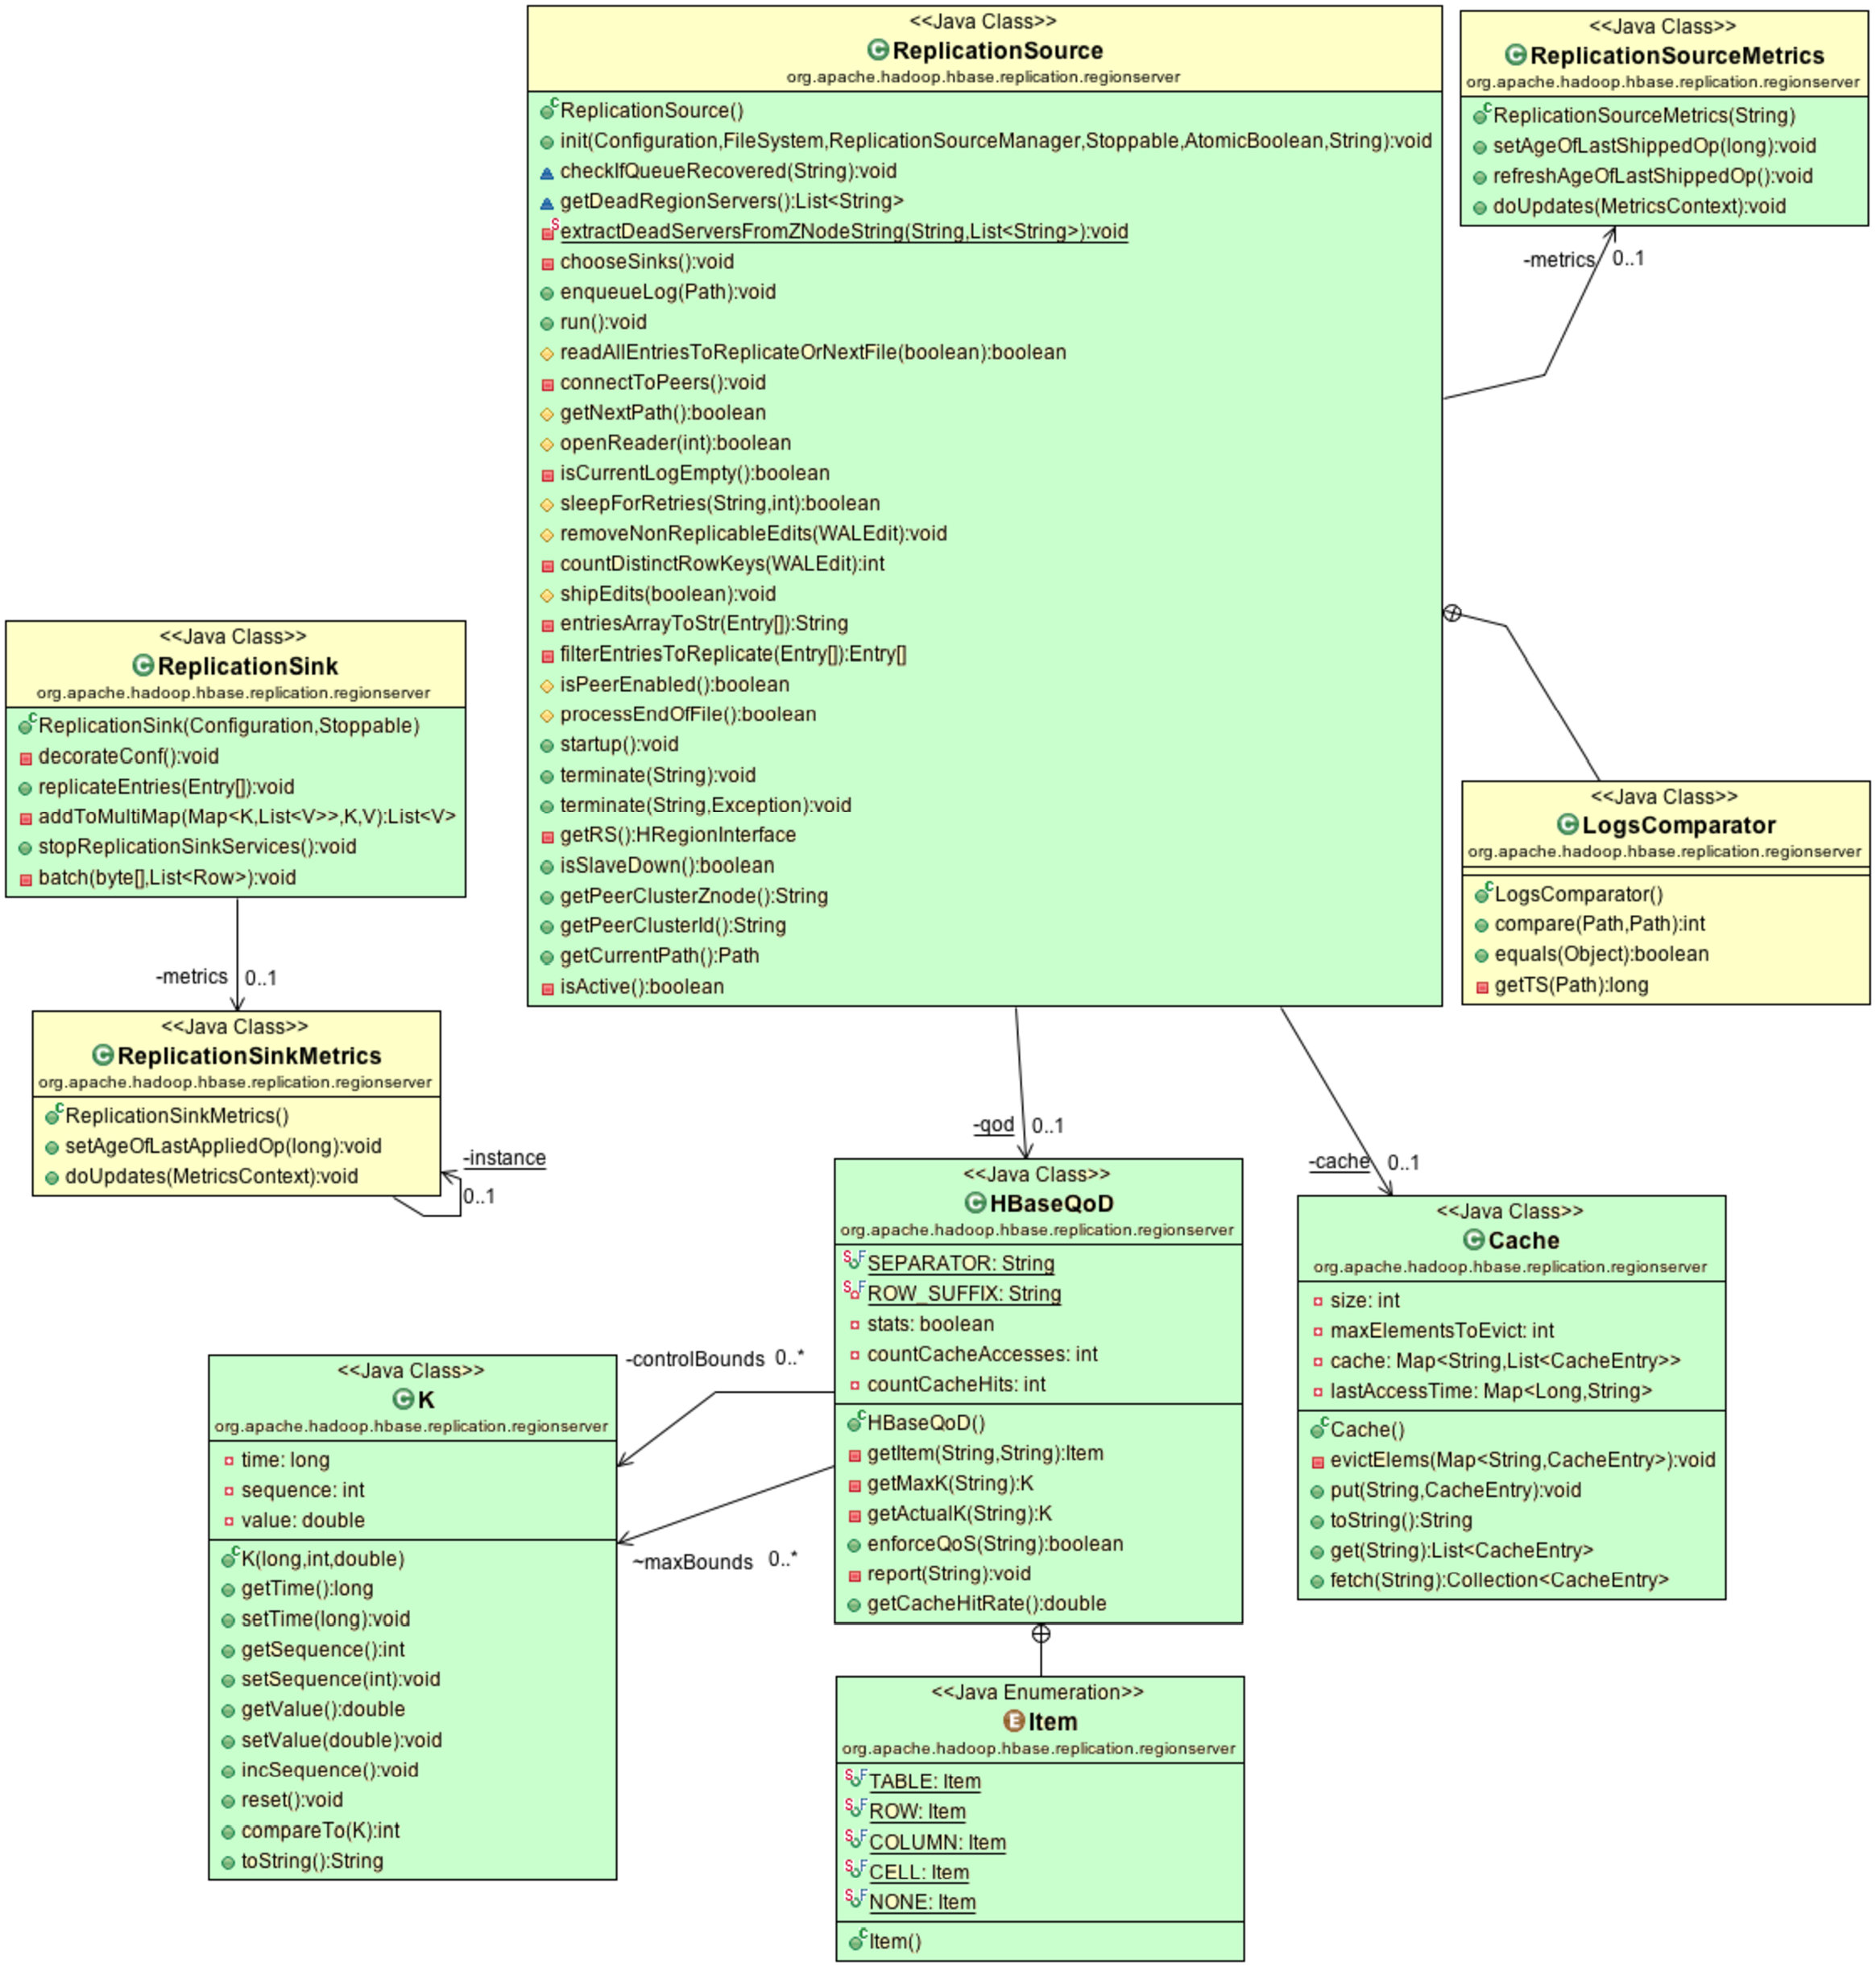
\includegraphics[width=1.0\linewidth]{figs/HBaseQoD-class-diagram.pdf}
\caption{HBase-QoD class diagram}
\label{fig-class-diagram}
\end{figure}



\section{Software Architecture}
%Class Diagram of relevant classes of each HBase instance and your new classes, and classes that have been modified in their interface/methods/public properties.
In the following Figure~\ref{fig-class-diagram} it is depicted the main class diagrams for the architecture solution. Highlighted diagrams in \emph{green} are classes we have introduced into the system or modified in the case of partially highlighted. The main components are the HBaseQoD and the function \emph{filterEntriesToReplicate} where resides the main Algorithm~\ref{algo1} for the consistency enforcement of data semantics we see in \ref{architecture:consistency}.


%this may fall into chapter 4, and is a way of making the bridge to the real implementation details in Chap.4.
Regarding operation grouping, the same logic applies to batches of operations which are grouped based on data dependencies or container-id most restrictive vector field (e.g sequence).


\subsection*{Summary}
This Chapter described the core aspects of our HBase-QoD proposal, addressing its architecture, regarding system, network and software components. We also described the relevant aspects that make consistency enforcement more flexible and aware of user/developer semantics, driven by QoD consistency vectors, followed by the operation/update grouping semantics also provided.

%This is the main outline of the architecture of the system. Next chapter digs into the details of the solution and its technical implementation. 


\newpage
\thispagestyle{empty}

  %%%%%%%%%%%%%%%%%%%%%%%%%%%%%%%%%%%%%%% -*- coding: utf-8; mode: latex -*- %%
  %
%%%%%                     IMPLEMENTATION
 %%%
  %

\chapter{Implementation}

\label{ch:implemenation}

\begin{quotation}
"Keep it simple, stupid" K-I-S-S, is an acronym as a design principle noted by the U.S. Navy in 1960. The KISS principle states that most systems work best if they are kept simple rather than made complex; therefore simplicity should be a key goal in design and unnecessary complexity should be avoided.
{\small\it -- Kelly Johnson, aircraft engineer (1910 - 1990)}
\end{quotation}

  %%%%%%%%%%%%%%%%%%%%%%%%%%%%%%%%%%%%%%%%%%%%%%%%%%%%%%%%%%%%%%%%%%%%%%%%%%%%%

This chapter deals with all the topics related to the implementation of the solution that was proposed in Chapter 3. Important points are reviewed and will explained in more detail such as the the working tools, the QoD module and the process follow to develop and introduce the necessary changes made into the original HBase implementation before this action took place. The chapter is organized as follows. Firstly we give an overview of the itinerary followed in~\ref{roadmap}. Section~\ref{proposal} describes the architecture of the existing and proposed system very briefly. In Section~\ref{integration} the inner-workings of the main extensions made are outlined, namely modifications to existing classes in HBase and addition of new ones to the source code of the system. That is, the QoD module and some of its most important aspects. In addition to that, in part~\ref{grouping} we also explain how to group updates and what are the benefits of it. Later, in section~\ref{method} the methodology used to develop the solution is described. The final section~\ref{summary-implementation} summarizes the chapter and some of the most important points made.

 %%%%%%%%%%%%%%%%%%%%%%%%%%%%%%%%%%%%%%%%%%%%%%%%%%%%%%%%%%%%%%%%%%%%%%%%%%%%%
  %
%%%%%                        SECTION
 %%%
  %
\section{Roadmap}\label{roadmap}
In distributed scenarios, Facebook is currently using HBase to manage very large number of messages across data centers for their users, and not Cassandra~\cite{FacebookHBase} That is because of the simplicity of consistency model, as well as the ability of HBase to handle both a short set of volatile data and an ever-growing amount, that rarely gets accessed more than once. More specifically, in their architecture reports, a Key for each element is the userID as RowKey, word as Column and messageID as Version and finally the value like offset of word in message (Data is sorted as \emph{userId, word, messageID} ). That implicitly means that searching for the top messageIDs of an specific user and word is easily supported, and therefore queries run faster in the backend.

With eventual consistency, updates and insertions are propagated asynchronously between clusters so Zookeeper is used for storing their positions in log files that hold the next log entry to be shipped in Hbase. To ensure cyclic replication (master to master) and prevent from copying same data back to the source, a sink location with remote procedure calls invoked is already into place with HBase. Therefore if we can control the edits to be shipped, we can also decide what is replicated, when or in other words how often. Keeping that in mind, we leverage the internal mechanisms of VFC$^{3}$ to tune HBase consistency, without requiring intrusion to the data schema and avoiding middle-ware overhead.

For filtering purposes, with our new proposal and implementation, we will enable administrators of the clusters to create quality-of-data policies that can analyze fetched data by inspecting some given bounds or semantics, and then receiving them on the master server at the other end of the replication chain if a match occurs. The term "Tunable" or "Enhanced" \emph{eventual consistency} is sparingly used across the text to describe the model presented on inter-site replication scenarios of HBase. The goal is providing an adaptive consistency model and based on Service Level Objectives agreed or defined previously by users or clients. The idea can be somehow similar to the "pluggable replication framework" proposed within the HBase community we reference in this text.


  %%%%%%%%%%%%%%%%%%%%%%%%%%%%%%%%%%%%%%%%%%%%%%%%%%%%%%%%%%%%%%%%%%%%%%%%%%%%%
  %
%%%%%                        SECTION
 %%%
  %

\section{Extensions to the HBase internal mechanisms}\label{proposal}
The initial approach follows built-in properties of HBase in regards to HDFS. We use the WALEdit data structure of Hbase rather than reinventing the wheel. A WALEdit structure contains information about the incoming updates to the tables in the system and it is later saved in the form of HLog entry, in that write ahead log as it needs to be be committed to persistent storage later, HDFS.

In Hbase we modify its inner workings by populating and sorting a custom priority queue of items to be replicated until at a later stage a thread is triggered to pick up one at a time and then copy the relevant entries into another queue that will ship the rows to the remote location with the usual HBase mechanism.

%% Start by presenting our model, constraints, data containers, and how things work (are enforced / evaluated )
The QoD paradigm implemented allows for entries to be evaluated prior to replication based on one or several of the three parameters in a three-dimensional vector K ($\theta$, $\sigma$, $\nu$), corresponding to Time, Sequence, Value respectively in our case. Secondly, we take care of updates that collide with previous ones (same keys but different values). They can also be checked for number of pending updates or value difference from previously replicated updates, and then shipped or kept on the data structure accordingly. The time constraint can be always validated every X seconds, and the other two constraints are validated through Algorithm.~\ref{algo1}, whenever updates arrive. For the work presented here we use Sequence ($\sigma$) as the main vector-field bound (\texttt{HBaseQoD.enforce(containerId)}).

  %%%%%%%%%%%%%%%%%%%%%%%%%%%%%%%%%%%%%%%%%%%%%%%%%%%%%%%%%%%%%%%%%%%%%%%%%%%%%
  %
%%%%%                     SECTION
 %%%
  %

\section{How to integrate a Quality of Data (QoD) module into HBase}\label{integration}

In Hbase it is necessary therefore to modify its inner workings by creating, populating and sorting a custom priority queue of items to be replicated. At a later stage, those items will be picked up by a thread which triggers replication one at time or by grouping them into a single operation. In order to do that, we devised a first experimentation with a vector-field data structure below described in Listing~\ref{lst:vector-listing}.

\begin{lstlisting}[caption={K.java},label={lst:vector-listing}]

package org.apache.hadoop.hbase.replication.regionserver;

	public class K implements Comparable<K> {
	    private long time;
	    private int sequence;
	    private double value;

	    public K(long time, int sequence, double value) {
	        this.time = time;
	        this.sequence = sequence;
	        this.value = value;
	    }

	    public long getTime() {
	        return time;
	    }

	    public void setTime(long time) {
	        this.time = time;
	    }

	    public int getSequence() {
	        return sequence;
	    }

	    public void setSequence(int sequence) {
	        this.sequence = sequence;
	    }

	    public double getValue() {
	        return value;
	    }

	    public void setValue(double value) {
	        this.value = value;
	    }

	    public void incSequence() {
	        this.sequence++;
	    }

	    public void reset() {
	        this.sequence = 0;
	        this.value = -1;
	        this.time = -1;
	    }

	    @Override
	    public int compareTo(K o) {
	        if (o.sequence > 0 && sequence > o.sequence)
	            return 1;

	        return 0;
	    }

	    @Override
	    public String toString() {
	        return "K(" + time + ", " + sequence + ", " + value + ")";
	    }
	}

\end{lstlisting}



%to pick up one at a time and then copy the relevant entries into another queue that will ship the rows to the remote location with the usual HBase mechanism.

%% Build up here on WAL, ReplicationSource, etc. Also architecture drawings.
In order to provide bounded consistency guarantees with QoD, we add it to the inner workings of Hbase. There are existing command line tools as CopyTable in HBase where one can manually define what is going to be replayed to the log and this is useful for cases where new replicas need to be put up to date or in disaster recovery too. We focus our implementation efforts into organising a list of items in memory (extending the original structure reflected for the updates to be shipped), where we can apply our QoD principles and directly enforce constraints. We do that by defining our bounded model over data which is indexed and queried by key (containerId), and can be enforced through time constraints (T), sequence (number of pending updates) and value ( percentage of changes). For the prototype just sequence. In other words \texttt{HBaseQoD.enforce(containerId)}.

% Keep building on it here. Talk about the WALPlayer and possibly how to replay messages but not only.
Every new update is checked for QoD and shipped for replication, or retained for later and immediate replication at the moment of reaching the QoD triggering condition defined at runtime by the developer. The QoD allows for entries to be evaluated by one or several of the three parameters as seen in vector field consistency \emph{K (time, sequence value)}~\cite{Santos:2007} Any new updates over previous ones (same data) can be also checked for number of pending updates or value difference from previously replicated update, and then shipped or kept on the data structure accordingly.

The original HBase architecture has built-in properties derived from the underlying HDFS layer. As part of it, the WALEdit data structure is used to store data temporarily before being replicated, useful to copy data between several HBase locations. The QoD algorithm (shown in Algorithm.~\ref{algo1}) uses that data structure, although we extend it to contain more meaningful information that help us in the management of the outgoing updates marked for replication.

% High-level algorithm we use to modify queued items for replication
\begin{algorithm*}
\caption{QoD high-level algorithm for filtering updates}
\label{algo1}
\begin{algorithmic}[1]
\REQUIRE $containerId$
\ENSURE $maxBound \neq 0$ and $controlBound \neq 0$
%\STATE $y \leftarrow 1$
\WHILE{$enforceQoD (containerId)$}
\IF{$getMaxK(containerId) = 0$}
\RETURN $true$
\ELSE[$getactualK(containerId)$]
\STATE $actualK(\sigma) \leftarrow actualK(\sigma)+1$
	\IF{$actualK(\sigma) \geq containerMaxK(\sigma)$}
	\STATE $actualK(\sigma) \leftarrow 0$
	\RETURN $true$
	\ELSE
	\RETURN $false$
	\ENDIF
\ENDIF
\ENDWHILE
\end{algorithmic}
\end{algorithm*}

  %%%%%%%%%%%%%%%%%%%%%%%%%%%%%%%%%%%%%%%%%%%%%%%%%%%%%%%%%%%%%%%%%%%%%%%%%%%%%
  %
%%%%%                         SECTION
 %%%
  %
\subsection{Operation Grouping}\label{grouping}
At the application level, it may be useful for HBase clients to enforce the same consistency level on groups of operations despite affected data containers having different QoD bounds associated. In other words, there may be specific situations where write operations need to be grouped so that they can be all handled at the same consistency level and propagated atomically to slave clusters. 

For example, publication of user statuses in social networks is usually handled at eventual consistency, but if they refer to new friends being added (e.g., an update to the data container holding the friends of a user), they should they should be handled at a stronger consistency level to ensure they are atomically visible along with the list of friends of the user in respect to the semantics we describe here.

In order to not violate QoD bounds and maintain consistency guarantees, all data containers of operations being grouped must be propagated either immediately after the block execution, or when any of the QoD bounds associated to the operations has been reached. When a block is triggered for replication, all respective QoD bounds are naturally reset. 

To enable this behavior we propose extending the HBase client libraries to provide atomically consistent blocks.
Namely, adding two new methods to HTable class in order to delimit the consistency blocks: \textit{startConsistentBlock} and \textit{endConsistentBlock}. Each block, through the method \textit{startConsistentBlock}, can be parameterized with one of the two options: i) \textit{IMMEDIATE}, which enforces stronger consistency for the whole block of operations within it; and ii) \textit{ANY}, which replicates a whole block as soon as any QoD vector field bound, associated with an operation inside the block is reached.

Next, in Listing~\ref{lst:group-listing} we provide an illustrative simple example of a social network where three containers with different consistency levels are modified. Note that we are not aiming at full transactional support, as it would be possible to change the same data containers modified by a set of grouped operations, at the same time, from other operations individually.

\begin{lstlisting}[language={java}, caption={Operation grouping},label={lst:group-listing}]
htable.startConsistentBlock(ConsistencyType.IMMEDIATE)
Put put1 = new Put(Bytes.toBytes("row1"));
put1.add(Bytes.toBytes("SocialNetTable"),Bytes.toBytes("status"), Bytes.toBytes("friend 12345 added"));

Put put2 = new Put(Bytes.toBytes("row2"));
put2.add(Bytes.toBytes("SocialNetTable"), Bytes.toBytes("friends"), Bytes.toBytes("12345"));

Put put3 = new Put(Bytes.toBytes("row3"));
put3.add(Bytes.toBytes("SocialNetTable"), Bytes.toBytes("wall"), Bytes.toBytes("12345 is now a friend"));

htable.put(put1);
htable.put(put2);
htable.put(put3);

htable.endConsistentBlock();
\end{lstlisting}

\subsection{Proposed scenario}
One of the key factors for having operations grouping working together with HBase-QoD is the depicted in Figure~\ref{fig-qod-grouping}. We can see that the operations that are grouped need to communicate over the network less often to other clusters, while arriving earlier in some cases than updates shipping as if several individual operations from location Cluster A were performed. This is due to the ability of HBase-QoD to deliver demanded updates in a consistent timely-fashion rather than on a per request arrival basis, which means possibly delaying the replication process by a fraction of the amount of communication that can be saved instead using the mentioned technique.

\begin{figure}[t]
\centering
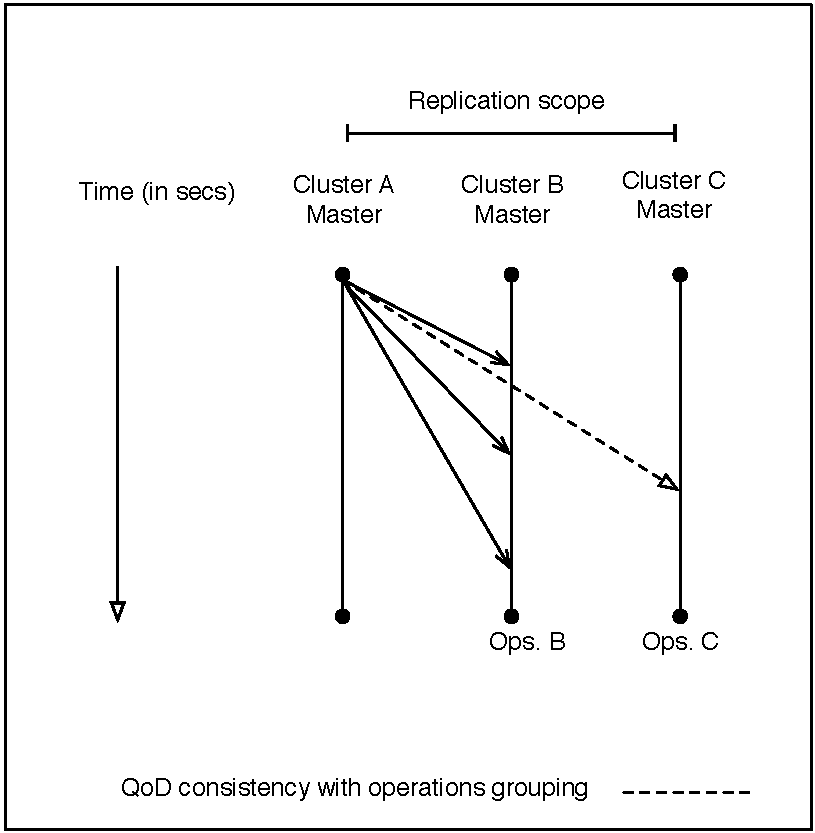
\includegraphics[scale=0.6]{figs/operation-grouping.pdf}
\caption{Resulting scenario of grouping operations in a time-lined based diagram using HBase-QoD versus a regular HBase deployment at Cluster B}
\label{fig-qod-grouping}
\end{figure}

Another experiment that has been conclusive in terms of grouping of operations is the comparison between different QoD levels, in the case of values for vector field K (-, $\sigma$, -). Setting the operation grouping for a small number of updates still shows that a timestamp in the receiving server is the same for every item in the group. The following set of operations is reflect in Figures~\ref{fig-shipping-grouping} and ~\ref{fig-receiving-grouping}. The same principle can be applied and has been demonstrated to work in the same fashion for different sets of containers.

%(table_name::columnFamily).

\begin{figure}[b]
\centering
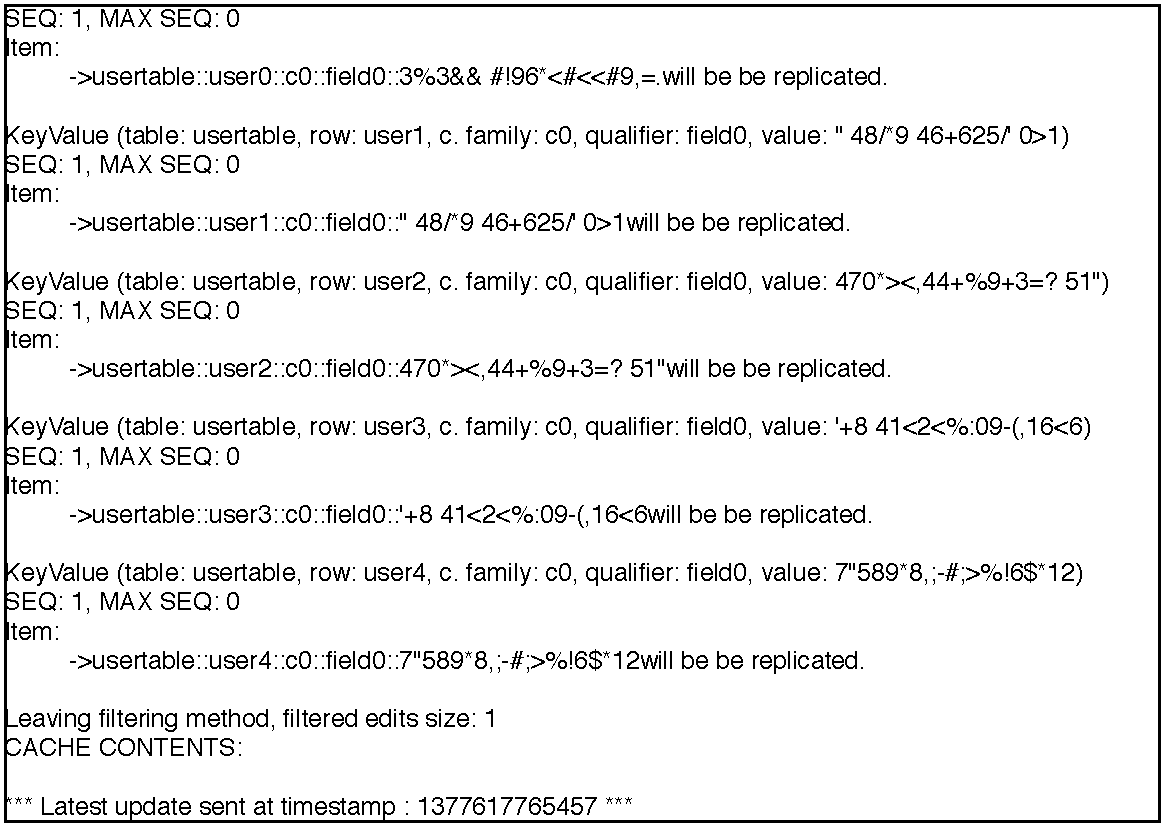
\includegraphics[scale=0.6]{figs/ginja2-grouping-send.pdf}
\caption{Sending from ginja-a2 to ginja-a1}
\label{fig-shipping-grouping}
\end{figure}

In the following Figure~\ref{fig-receiving-grouping}, we observe how the timestamp for each of the items replicated from the grouped operation have the same timestamp (\textbf{1377617765557}) at the receiving side on ginja-a1. That ensures they have arrived at the same time, and actually we verify the correctness of the experiment by leveraging internal HBase mechanisms that are currently being already used to list statistics of the age of updates sent and/or receive. At the sending side on the other hand, each update is grouped until finally they are all due to be replicated as a whole and therefore printing the timestamp only in order to comply with the reality.

\begin{figure}[t]
\centering
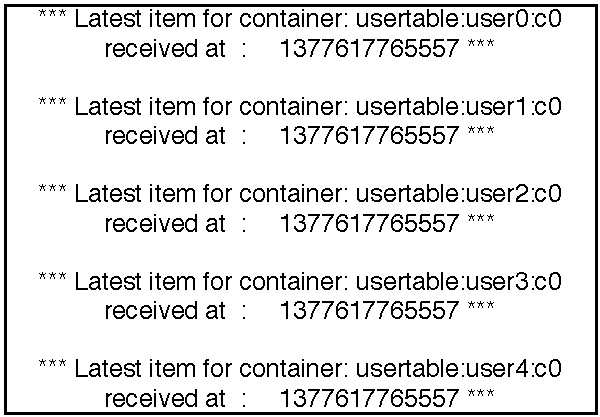
\includegraphics[scale=.6]{figs/ginja1-grouping-receive.pdf}
\caption{Receiving from ginja-a2 in ginja-a1}
\label{fig-receiving-grouping}
\end{figure}
 


  %
 %%%
%%%%%                           SECTION
  %
  %%%%%%%%%%%%%%%%%%%%%%%%%%%%%%%%%%%%%%%%%%%%%%%%%%%%%%%%%%%%%%%%%%%%%%%%%%%%%


\section{Implementation remarks}\label{summary-implementation}

%%% Local Variables: 
%%% mode: latex
%%% TeX-master: "tese"
%%% End: 
               % the implementation details

  %%%%%%%%%%%%%%%%%%%%%%%%%%%%%%%%%%%%%%%%%%%%%%%%%%%%%%%%%%%%%%%%%%%%%%%%%%%%%
  %

%%%%%                 P A R T E   I V  --  Evaluation
 %%%
  %

%\part{Part}
\thispagestyle{empty}
%\vbox to\textheight{
%\vfil
%\chapter*{Experiments and testing}
\thispagestyle{empty}

%The chapter describes all the experiments and tests conducted up to the date of the delivery of the thesis.

%}
\newpage
\thispagestyle{empty}

  %%%%%%%%%%%%%%%%%%%%%%%%%%%%%%%%%%%%%%% -*- coding: utf-8; mode: latex -*- %%
  %
%%%%%                       CHAPTER
 %%%
  %

% $Id: 3100-nihil-molestiae.tex,v 1.1 2007/11/23 09:52:43 david Exp $
% $Log: 3100-nihil-molestiae.tex,v $
% Revision 1.1  2007/11/23 09:52:43  david
% *** empty log message ***
%
%

  %%%%%%%%%%%%%%%%%%%%%%%%%%%%%%%%%%%%%%%%%%%%%%%%%%%%%%%%%%%%%%%%%%%%%%%%%%%%%
  %
%%%%%                    HEAD MATTER
 %%%
  %

\chapter{Evaluation}
%\addcontentsline{lof}{chapter}{\thechapter\quad Nihil Molestiae}
%\addcontentsline{lot}{chapter}{\thechapter\quad Nihil Molestiae}
\label{ch:evaluation}

%\begin{quotation}
%  {\small\it }
%
%{\small\it -- }
%\end{quotation}



  %%%%%%%%%%%%%%%%%%%%%%%%%%%%%%%%%%%%%%%%%%%%%%%%%%%%%%%%%%%%%%%%%%%%%%%%%%%%%
  %
%%%%%                        FIRST SECTION
 %%%
  %

\section{Testbed}
During evaluation of the QoD prototype a test-bed with several HBase cluster has been deployed at INESC-ID and IST in Lisbon, some of them with an HBaseQoD-enabled engine for quality of data between replicas, and others running a regular implementation of HBase 0.94.8. All tests were conducted using 6 machines with an Intel Core i7-2600K CPU at 3.40GHz, 11926MB of available RAM memory, and HDD 7200RPM SATA 6Gb/s 32MB cache, connected by 1 Gigabit LAN and we expect to continue obtaining results using a network tool as~\cite{netem:2005} for delaying and simulating network bandwidth and latency between a distant set of locations. We are also currently trying to confirm that the appropriate QoD does have a positive impact when bounding staleness (monitoring time an pending updates, instead of number of updates) with varying delays, but not now due to space constraints in this text, we do not present it. Even though, it is obvious this will just spread replication activity in time, but expecting a reduced max-value on each network peak-load observed.


\section{Experiments}

\begin{figure}[h]
\centering
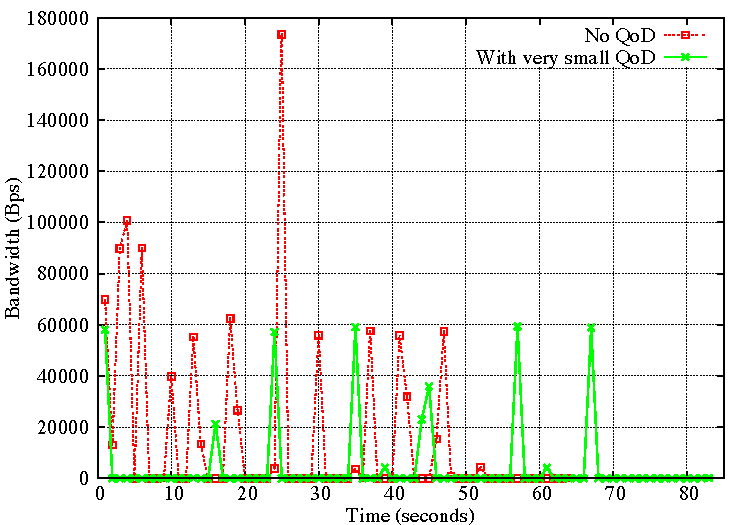
\includegraphics[width=0.8\textwidth]{figs/bandwidth.pdf}
\caption{Bandwidth usage and replication frequency for a typical workload with and very small HBase-QoD constraint for K($\sigma$)}
\label{fig-bw-freq}
\end{figure}

In Figure~\ref{fig-bw-freq} for a very small QoD of K using $\sigma$ we realize that there is a lower limit where latency can not be reduced any further. We have measured that same value in the subsequent Figure~\ref{fig-bandwidth-worloada-modified} with a larger QoD of K using $\sigma$ = 0.5\%. Recall this means the percentage of records allowed to be modified, or of updates applied in relation to total number of records, before replication is triggered (a very small value, where strict consistency would mean 0.00\%).

We can see the bandwidth peaks and therefore measure average usage of the former, which decreases with the increase of the QoD bound in the order of magnitude of 1MB per second as we experimentally verify from the graphs obtained. That is due to the batching of updates in our vector model, so items are not replicated until one of the constraints time, sequence or value is met. Basically, overall we can see less communication between clusters at replication time increasing QoD, which is a good measurement of how one can optimize bandwidth. During that time then we take advantage of our caching mechanisms inside QoD while sending all the information demanded in a timely fashion once data becomes necessary to the application.

%In Figure 1, we appreciated that our QoD helps to control peak bounds of updates, and therefore the eventual consistency approach of leaving replication of the items at the odds of the RPC mechanisms of the system in question. We %can control that, and the graph shows how a maximum threshold of around 1000 is constantly reached for the modified version of HBase, but no more. Obviously the timespan of updates with QoD might be longer depending of the values %chosen, but that is a built-in property of our work on purpose for only propagating updates when they are strictly necessary and to satisfy a given SLO.

\begin{figure}[h]
\centering
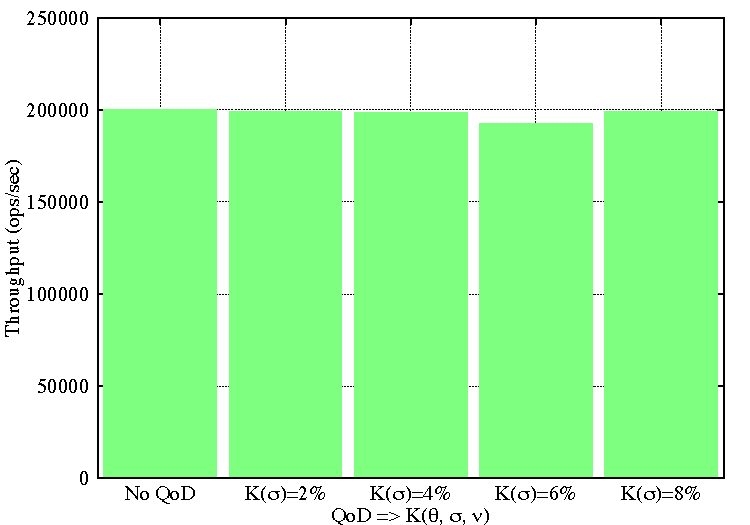
\includegraphics[width=0.8\linewidth]{figs/throughput.pdf}
\caption{Throughput for several QoD configurations}
\label{fig-throughput}
\end{figure}
We also confirm the QoD does not hurt performance as we observe from the throughput achieved for the several levels of QoD chosen during the evaluation of the throughput achieve with the benchmark for our modified version with HBase=QoD enabled, Figure~\ref{fig-throughput}. The differences in throughput are irrelevant and mostly due to noise in the network, that is the conclusion after obtaining similar results to that one in several rounds of tests with the same input workload on the data store.

Next we conducted as shown in Figure~\ref{fig-cpu}, and \emph{dstat} presents, an experiment to monitor the CPU usage using HBase-QoD. CPU consumption and performance remains roughly the same and therefore stable in the cluster machines as can be appreciated.
\begin{figure}[h]
\centering
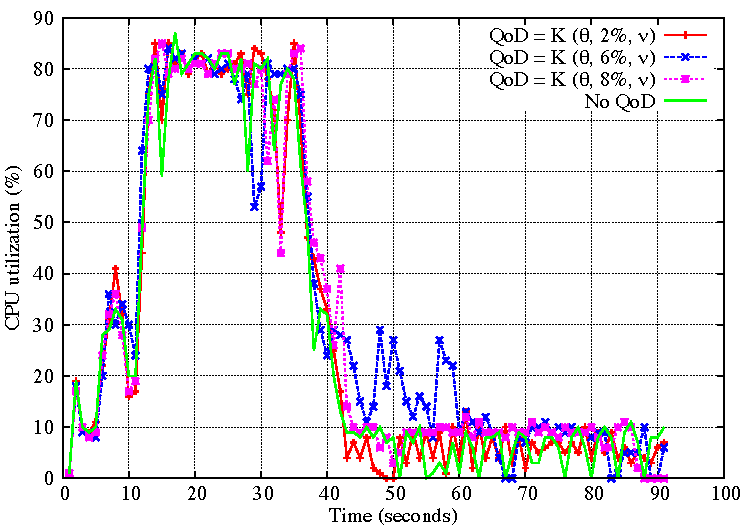
\includegraphics[width=0.8\linewidth]{figs/cpu.pdf}
\caption{CPU usage over time with QoD enabled}
\label{fig-cpu}
\end{figure}

%In Figure 4 (for batches of updates of 5M) we can see the bandwidth peaks and therefore measure average usage of the former, which decreases with the increase of the QoD bound in the order of magnitude of 1MB per second as we %experimentally verify from the graphs obtained. That is due to the batching of updates in our vector model, so items are not replicated until one of the constraints time, sequence or value is met. Basically, overall we can see %less communication between clusters at replication time increasing QoD, which is a good measurement of how one can optimize bandwidth while non-key data semantics are presented to the application at a required instant in time but %not earlier if not critical. During that time then we take advantage of our caching mechanisms inside QoD while sending all the information demanded in a timely fashion once data becomes necessary to the application.

We have also taken measurements for the following workloads obtaining results as follows:

\subsection{Workloads for YCSB}

We have tested our implementation in HBase with several built-in workloads from YCSB plus one customer workload with 100\% writes to stress the database intensively as the target updates in the social network previously described is about changes and new insertions.

Figure~\ref{fig-bandwidth-worloada} shows three different sets of Qualities of Data for the same workload (A):

\begin{enumerate}
\item{YCSB workload A (R/W - 50/50)}
	\begin{itemize}
		\item No QoD enforced.
		\item QoD fulfillment of $\sigma$=0.5\% of total updates to be replicated.
		\item QoD fulfillment of $\sigma$=2\% of total updates to be replicated.
	\end{itemize}

During the execution of the workload A, in Figure~\ref{fig-bandwidth-worloada}, the highest peaks in replication traffic are observed without any type of QoD, i.e. just using plain HBase. This is due to the nature of eventual consistency itself and the buffering mechanisms in HBase.

With a QoD enabled as shown in the other two graphs, we rather control traffic of updates from being unbounded to a limited amount, accordingly to save resources' utilization, while suiting applications that require small amounts of information to be only propagated as a group, when they are just needed.

We observe that higher QoD requires replication traffic less frequently, although interactions reach higher values on Bytes as they need to send more data. Small QoD optimizes the usage of resources while sending priority updates more frequently (this could be the case of wall posts in a social network).

\begin{figure*}
\centering
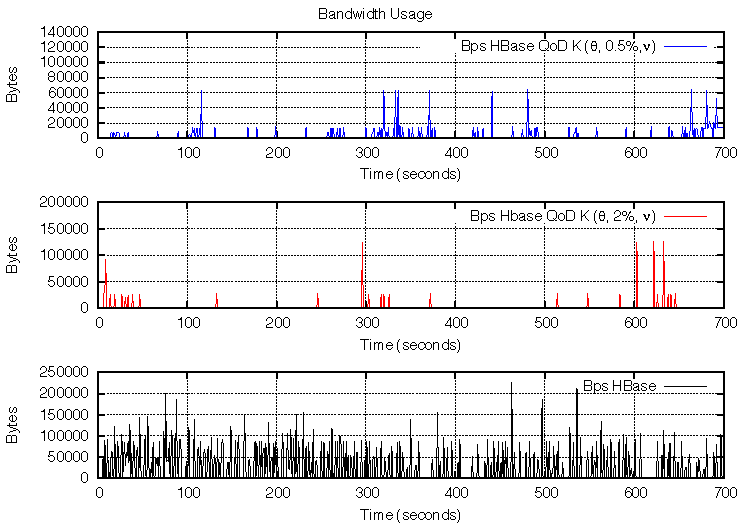
\includegraphics[width=0.8\linewidth]{figs/plot-packets-size-workloada-allbounds-latest.pdf}
\caption{Bandwidth usage for Workload A using 5M records using QoD bounds of 0.5 and 2\% in the $\sigma$ of K.}
\label{fig-bandwidth-worloada}
\end{figure*}

\item{YCSB workload A modified (R/W - 0/100)}
	\begin{itemize}
		\item No QoD enforced.
		\item QoD fulfillment of $\sigma$=0.5\% of total updates to be replicated.	% 25K updates (5M total)
		\item QoD QoD fulfillment of $\sigma$=2\% of total updates to be replicated.  % 100K updates (5M total)
	\end{itemize}
\end{enumerate}

\begin{figure*}
\centering
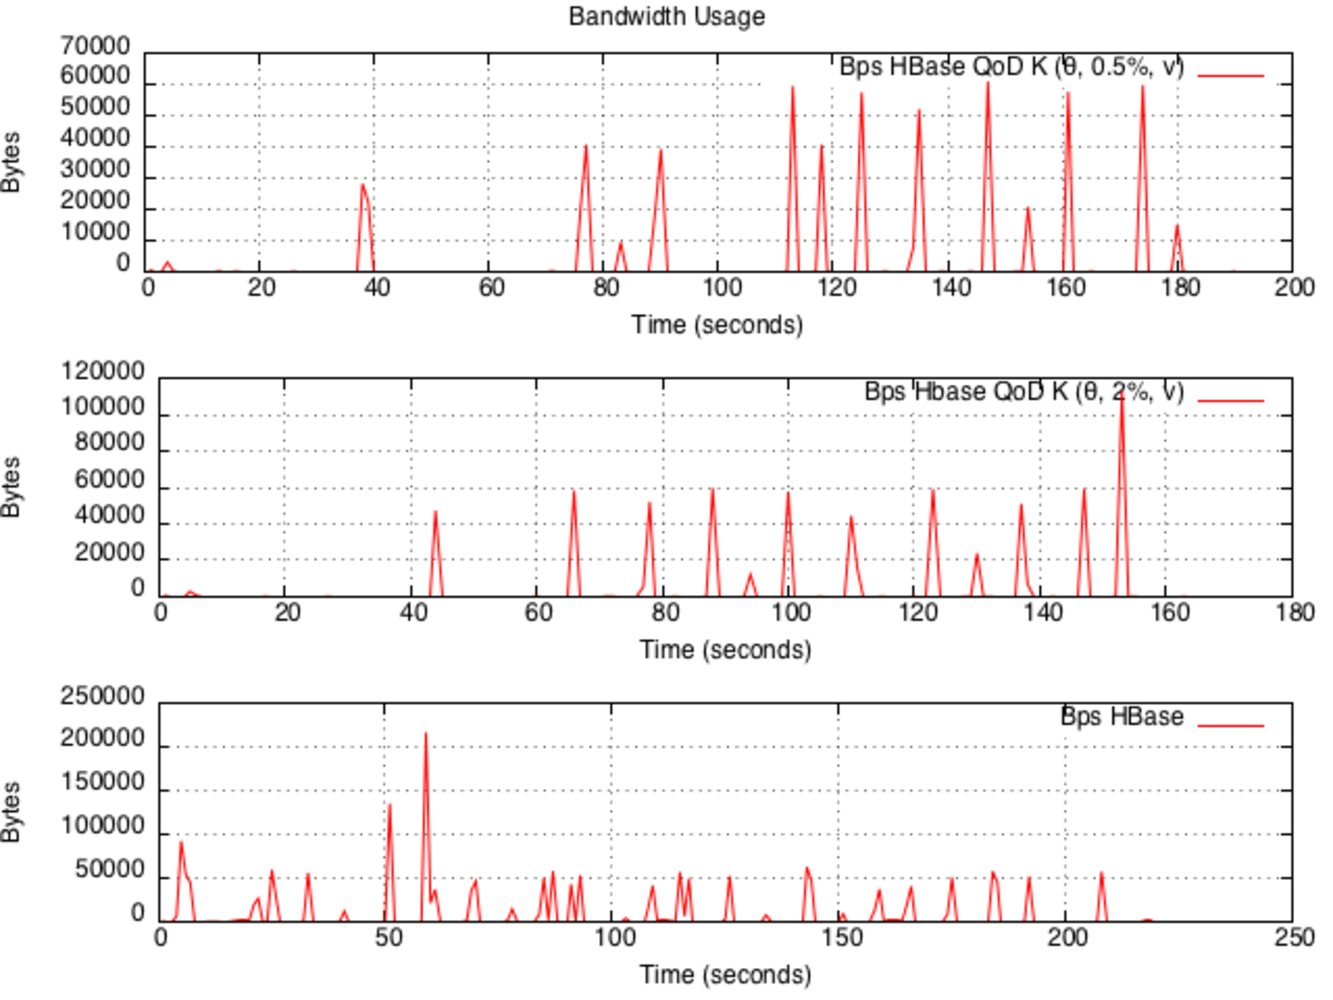
\includegraphics[width=0.8\linewidth]{figs/plot-packets-size-workloada-modified-allbounds-30threads.pdf}
\caption{Bandwidth usage for Workload A-Modified using 5M records using QoD bounds of 0.5 and 2\% in the $\sigma$ of K.}
\label{fig-bandwidth-worloada-modified}
\end{figure*}

In Figure ~\ref{fig-bandwidth-worloada-modified} we can see how a write intensive workload performs using a QoD. Similar results are expected and later also confirmed in this graph (please note the scale of the Y axis is modified in order to show the relevant difference in Bytes more accurately).
  For smaller QoD (0.5\%) we see lower peaks in bandwidth usage, as well as in the following measurement used (2.0\%). Finally HBase with no modifications shows a much larger number of Bytes when coming to maximum bandwidth consumption.
 
 Note we are not measuring, or find relevant, in any of these scenarios, to realize any kind of claims based on average bandwidth usage. The principal source of motivation of the paper is to find a way of controlling the usage of the resources in a data center, by ensuring a uniform distribution of replication of updates across time. Also, to be able to trade strong consistency for groups of operations treated atomically, for shipment to the destination cluster location at a given point in time, or when the data-semantics bound is reached. 


                 % Evaluation section
  %%%%%%%%%%%%%%%%%%%%%%%%%%%%%%%%%%%%%%% -*- coding: utf-8; mode: latex -*- %%
  %
%%%%%                       CHAPTER
 %%%
  %

% $Id: 3200-adipisci-velit.tex,v 1.2 2007/11/23 10:14:56 david Exp $
% $Log: 3200-adipisci-velit.tex,v $
% Revision 1.2  2007/11/23 10:14:56  david
% Bug fixes galore.
%
% Revision 1.1  2007/11/23 09:52:43  david
% *** empty log message ***
%
%

  %%%%%%%%%%%%%%%%%%%%%%%%%%%%%%%%%%%%%%%%%%%%%%%%%%%%%%%%%%%%%%%%%%%%%%%%%%%%%
  %
%%%%%                    HEAD MATTER
 %%%
  %

\chapter{Conclusion}
%\addcontentsline{lof}{chapter}{\thechapter\quad Nihil Molestiae}
%\addcontentsline{lot}{chapter}{\thechapter\quad Nihil Molestiae}
\label{ch:conclusion}

%\begin{quotation}
%  {\small\it Neque porro quisquam est qui dolorem ipsum quia dolor sit amet, consectetur, adipisci velit...}
%
%{\small\it -- Cerico}
%\end{quotation}



  %%%%%%%%%%%%%%%%%%%%%%%%%%%%%%%%%%%%%%%%%%%%%%%%%%%%%%%%%%%%%%%%%%%%%%%%%%%%%
  %
%%%%%                        FIRST SECTION.
 %%%
  %

\section{Concluding remarks}

The work here presented is therefore useful and applicable as flexible consistency model to cloud data stores in cases where bandwidth is precious and cost savings mandatory. Applied to the core of HBase for inter-datacenter scenarios, it provides users and applications with just the quality of data requested. On the other hand, administrators and developers can easily tune the bounds and framework in order to perform replication in a more fine-grained an timely-fashion. The same principle applies to cyclic multi-master scenarios, where each master acts as master and slave all at once. Although we did not test that or configure it in our slaves as we did find it critical in order to provide a feasible proof of concept for the proposal. In the future that would also be a good experiment to perform as well as testing with different set ups on Amazon EC2. To conclude, we have reviewed the most well-known and state of the art in replication for distributed systems, outlined the advantages and disadvantages of each of them. Following that, we performed a deeper introspection into the mechanisms of the selected cloud data store in questions for this work, HBase, where we identify its weaknesses (including currently missing features) and introduce our work later to realize the cost savings obtained in the Evaluation section. This paragraph concludes the thesis. Finally, we believe in the re-usability and possibility to extend and adapt the framework to other cloud data stores, so a wider choice of consistency guarantees can be provided on top of our implementation if further required by applications.

  %%%%%%%%%%%%%%%%%%%%%%%%%%%%%%%%%%%%%%%%%%%%%%%%%%%%%%%%%%%%%%%%%%%%%%%%%%%%%

%%% Local Variables: 
%%% mode: latex
%%% TeX-master: "tese"
%%% End: 


  %%%%%%%%%%%%%%%%%%%%%%%%%%%%%%%%%%%%%%%%%%%%%%%%%%%%%%%%%%%%%%%%%%%%%%%%%%%%%
  %
%%%%%                        SPECIAL
 %%%
  %
%\bibliographystyle{authordate3}             % Bibliography
%\bibliographystyle{apacitex}
\bibliographystyle{chicago}
\bibliography{MasterBibliographyThesis}	
%---------------------------------------------------------------------------
%\begin{singlespace}
%\printindex[autx]\cleardoublepage            % Author index (apacitex)
%\end{singlespace}

  %%%%%%%%%%%%%%%%%%%%%%%%%%%%%%%%%%%%%%%%%%%%%%%%%%%%%%%%%%%%%%%%%%%%%%%%%%%%%
  %
%%%%%                         APPENDIX
 %%%
  %

%\part{Appendices}
\appendix

%\input{}         % commodo consequat

%\begin{singlespace}
%\printnomenclature\cleardoublepage               % Glossary
%\end{singlespace}


  %%%%%%%%%%%%%%%%%%%%%%%%%%%%%%%%%%%%%%%%%%%%%%%%%%%%%%%%%%%%%%%%%%%%%%%%%%%%%
  %
%%%%%                         SPECIAL
 %%%
  %
\begin{singlespace}

\def\indexname{Index}             % Index
\printindex\cleardoublepage

\end{singlespace}

\end{document}

  %
 %%%
%%%%%                          THE END
  %
  %%%%%%%%%%%%%%%%%%%%%%%%%%%%%%%%%%%%%%%%%%%%%%%%%%%%%%%%%%%%%%%%%%%%%%%%%%%%%
